\documentclass[manuscript,screen,review,anonymous,nonacm]{acmart}

\usepackage{booktabs,graphicx}
\usepackage[capitalise,noabbrev]{cleveref}
\graphicspath{{../figures/}}
% Generated by Sher/paper/make_numbers.py from the repo's result files. Do not edit by hand.
\newcommand{\hmLlamaItems}{387}  % results/hedge_measure_v2/summary.txt
\newcommand{\hmLlamaSamples}{1{,}161}  % results/hedge_measure_v2/summary.txt
\newcommand{\hmLlamaKappa}{0.62}  % results/hedge_measure_v2/summary.txt
\newcommand{\hmLlamaObsUnk}{0.48}  % results/hedge_measure_v2/summary.txt primary cells
\newcommand{\hmLlamaObsKnown}{0.43}  % results/hedge_measure_v2/summary.txt primary cells
\newcommand{\hmLlamaPopUnk}{0.13}  % results/hedge_measure_v2/summary.txt primary cells
\newcommand{\hmLlamaPopKnown}{0.00}  % results/hedge_measure_v2/summary.txt primary cells
\newcommand{\hmLlamaPopEff}{$+$0.39}  % results/hedge_measure_v2/summary.txt primary pop
\newcommand{\hmLlamaPopEffCI}{[$+$0.33, $+$0.45]}  % results/hedge_measure_v2/summary.txt
\newcommand{\hmLlamaKnowEff}{$+$0.09}  % results/hedge_measure_v2/summary.txt primary know
\newcommand{\hmLlamaKnowEffCI}{[$+$0.03, $+$0.15]}  % results/hedge_measure_v2/summary.txt
\newcommand{\hmLlamaDiff}{$+$0.30}  % results/hedge_measure_v2/summary.txt primary pop-know
\newcommand{\hmLlamaDiffCI}{[$+$0.20, $+$0.40]}  % results/hedge_measure_v2/summary.txt
\newcommand{\hmLlamaRegexRecall}{0.99}  % results/hedge_measure_v2/summary.txt
\newcommand{\hmLlamaRegexDiff}{$+$0.43}  % results/hedge_measure_v2/summary.txt regex on 96-token replies pop-know
\newcommand{\hmLlamaSecDiff}{$+$0.31}  % results/hedge_measure_v2/summary.txt secondary pop-know
\newcommand{\hmQwenKappa}{0.30}  % results/hedge_measure_v2/summary.txt qwen
\newcommand{\hmQwenObsUnk}{0.05}  % results/hedge_measure_v2/summary.txt qwen primary obscure-unknown
\newcommand{\hmQwenRegexObsUnk}{0.18}  % results/hedge_measure_v2/summary.txt qwen regex obscure-unknown
\newcommand{\hmQwenSecObsUnk}{0.32}  % results/hedge_measure_v2/summary.txt qwen secondary obscure-unknown
\newcommand{\hmGemmaKappa}{0.47}  % results/hedge_measure_v2/summary.txt gemma
\newcommand{\hmGemmaObsUnk}{0.05}  % results/hedge_measure_v2/summary.txt gemma primary obscure-unknown
\newcommand{\hmGemmaRegexObsUnk}{0.07}  % results/hedge_measure_v2/summary.txt gemma regex obscure-unknown
\newcommand{\hmGemmaSecObsUnk}{0.22}  % results/hedge_measure_v2/summary.txt gemma secondary obscure-unknown
\newcommand{\hmMistralKappa}{0.39}  % results/hedge_measure_v2/summary.txt mistral
\newcommand{\hmMistralObsUnk}{0.10}  % results/hedge_measure_v2/summary.txt mistral primary obscure-unknown
\newcommand{\hmMistralRegexObsUnk}{0.21}  % results/hedge_measure_v2/summary.txt mistral regex obscure-unknown
\newcommand{\hmMistralSecObsUnk}{0.25}  % results/hedge_measure_v2/summary.txt mistral secondary obscure-unknown
\newcommand{\faLlamaRegexPop}{0.63}  % results/factorial_4models/effects.csv llama hedge_rate pop
\newcommand{\faLlamaRegexKnow}{0.19}  % results/factorial_4models/effects.csv llama hedge_rate know
\newcommand{\faLlamaRegexDiff}{$+$0.44}  % results/factorial_4models/effects.csv llama hedge_rate diff
\newcommand{\hjLlamaDiff}{$+$0.13}  % results/hedge_judge/summary.txt llama corrected pop - know
\newcommand{\hjQwenRecall}{0.10}  % results/hedge_judge/summary.txt
\newcommand{\hjGemmaRecall}{0.14}  % results/hedge_judge/summary.txt
\newcommand{\hjMistralRecall}{0.14}  % results/hedge_judge/summary.txt
\newcommand{\entLlamaPop}{$+$0.51}  % results/factorial_4models/effects.csv llama entropy pop
\newcommand{\entLlamaKnow}{$+$2.14}  % results/factorial_4models/effects.csv llama entropy know
\newcommand{\entLlamaKnowCI}{[$+$2.05, $+$2.23]}  % results/factorial_4models/effects.csv llama entropy know CI
\newcommand{\entLlamaPopCI}{[$+$0.42, $+$0.61]}  % results/factorial_4models/effects.csv llama entropy pop CI
\newcommand{\entQwenPop}{$-$0.02}  % results/factorial_4models/effects.csv qwen entropy pop
\newcommand{\entQwenKnow}{$+$1.23}  % results/factorial_4models/effects.csv qwen entropy know
\newcommand{\entQwenKnowCI}{[$+$1.13, $+$1.33]}  % results/factorial_4models/effects.csv qwen entropy know CI
\newcommand{\entQwenPopCI}{[$-$0.12, $+$0.08]}  % results/factorial_4models/effects.csv qwen entropy pop CI
\newcommand{\entGemmaPop}{$+$0.09}  % results/factorial_4models/effects.csv gemma entropy pop
\newcommand{\entGemmaKnow}{$+$1.08}  % results/factorial_4models/effects.csv gemma entropy know
\newcommand{\entGemmaKnowCI}{[$+$1.03, $+$1.13]}  % results/factorial_4models/effects.csv gemma entropy know CI
\newcommand{\entGemmaPopCI}{[$+$0.05, $+$0.14]}  % results/factorial_4models/effects.csv gemma entropy pop CI
\newcommand{\entMistralPop}{$+$0.30}  % results/factorial_4models/effects.csv mistral entropy pop
\newcommand{\entMistralKnow}{$+$1.41}  % results/factorial_4models/effects.csv mistral entropy know
\newcommand{\entMistralKnowCI}{[$+$1.33, $+$1.50]}  % results/factorial_4models/effects.csv mistral entropy know CI
\newcommand{\entMistralPopCI}{[$+$0.21, $+$0.38]}  % results/factorial_4models/effects.csv mistral entropy pop CI
\newcommand{\hrLlamaObsUnk}{0.85}  % results/factorial_4models/cells.csv llama hedge_rate uncertain/Unknown
\newcommand{\faLlamaN}{2{,}303}  % results/factorial_4models/cells.csv llama sum of cell n (HighlyKnown+Unknown)
\newcommand{\hrQwenObsUnk}{0.09}  % results/factorial_4models/cells.csv qwen hedge_rate uncertain/Unknown
\newcommand{\faQwenN}{2{,}392}  % results/factorial_4models/cells.csv qwen sum of cell n (HighlyKnown+Unknown)
\newcommand{\hrGemmaObsUnk}{0.07}  % results/factorial_4models/cells.csv gemma hedge_rate uncertain/Unknown
\newcommand{\faGemmaN}{2{,}282}  % results/factorial_4models/cells.csv gemma sum of cell n (HighlyKnown+Unknown)
\newcommand{\hrMistralObsUnk}{0.13}  % results/factorial_4models/cells.csv mistral hedge_rate uncertain/Unknown
\newcommand{\faMistralN}{2{,}378}  % results/factorial_4models/cells.csv mistral sum of cell n (HighlyKnown+Unknown)
\newcommand{\loGemmaPop}{$+$1.79}  % results/factorial_4models/effects.csv gemma hedge_logodds pop
\newcommand{\loGemmaKnow}{$-$0.32}  % results/factorial_4models/effects.csv gemma hedge_logodds know
\newcommand{\loLlamaPop}{$+$2.93}  % results/factorial_4models/effects.csv llama hedge_logodds pop
\newcommand{\loLlamaKnow}{$+$3.05}  % results/factorial_4models/effects.csv llama hedge_logodds know
\newcommand{\scPopKnownPairs}{55}  % results/unireps_checks/check1_pairs.csv
\newcommand{\scPopKnownGap}{$+$0.76}  % results/unireps_checks/check1_pairs.csv mean d_hedge pop_given_known
\newcommand{\scPopKnownGapSurface}{$+$0.43}  % results/unireps_checks/summary.txt
\newcommand{\scPopKnownGapSurfaceCI}{[$+$0.18, $+$0.69]}  % results/unireps_checks/summary.txt
\newcommand{\scNonInferN}{36}  % results/unireps_checks/summary.txt
\newcommand{\scNonInferGap}{$+$0.79}  % results/unireps_checks/summary.txt
\newcommand{\scPoolPop}{$-$1.87}  % results/unireps_checks/summary.txt M1 logpop_z (hedge GLM)
\newcommand{\scPoolPopSurface}{$-$1.79}  % results/unireps_checks/summary.txt M2 logpop_z (hedge GLM)
\newcommand{\stLlamaDose}{1}  % results/direction_reuse_v2/llama/summary.txt
\newcommand{\stLlamaLayer}{17}  % results/direction_reuse_v2/llama/summary.txt l*
\newcommand{\stLlamaLayers}{32}  % results/direction_reuse_v2/llama/summary.txt layers
\newcommand{\stLlamaN}{150}  % results/direction_reuse_v2/llama/summary.txt n
\newcommand{\stLlamaNone}{0.02}  % results/direction_reuse_v2/llama/summary.txt none
\newcommand{\stLlamaFam}{0.29}  % results/direction_reuse_v2/llama/summary.txt own_fam
\newcommand{\stLlamaKnow}{0.09}  % results/direction_reuse_v2/llama/summary.txt inst_know
\newcommand{\stLlamaBase}{0.02}  % results/direction_reuse_v2/llama/summary.txt base_fam
\newcommand{\stLlamaRand}{0.03}  % results/direction_reuse_v2/llama/summary.txt mean of random0-4
\newcommand{\stLlamaDH}{$+$0.20}  % results/direction_reuse_v2/llama/summary.txt DD hedge
\newcommand{\stLlamaDHCI}{[$+$0.14, $+$0.27]}  % results/direction_reuse_v2/llama/summary.txt
\newcommand{\stLlamaDE}{$-$0.03}  % results/direction_reuse_v2/llama/summary.txt DD entropy
\newcommand{\stLlamaDECI}{[$-$0.11, $+$0.05]}  % results/direction_reuse_v2/llama/summary.txt
\newcommand{\stLlamaEntNone}{0.82}  % results/direction_reuse_v2/llama/summary.txt entropy none
\newcommand{\stLlamaEntKnow}{1.23}  % results/direction_reuse_v2/llama/summary.txt entropy inst_know
\newcommand{\stLlamaEntFam}{1.26}  % results/direction_reuse_v2/llama/summary.txt entropy own_fam
\newcommand{\stGemmaDose}{4}  % results/direction_reuse_v2/gemma9b/summary.txt
\newcommand{\stGemmaLayer}{23}  % results/direction_reuse_v2/gemma9b/summary.txt l*
\newcommand{\stGemmaLayers}{42}  % results/direction_reuse_v2/gemma9b/summary.txt layers
\newcommand{\stGemmaN}{150}  % results/direction_reuse_v2/gemma9b/summary.txt n
\newcommand{\stGemmaNone}{0.00}  % results/direction_reuse_v2/gemma9b/summary.txt none
\newcommand{\stGemmaFam}{0.22}  % results/direction_reuse_v2/gemma9b/summary.txt own_fam
\newcommand{\stGemmaKnow}{0.00}  % results/direction_reuse_v2/gemma9b/summary.txt inst_know
\newcommand{\stGemmaBase}{0.00}  % results/direction_reuse_v2/gemma9b/summary.txt base_fam
\newcommand{\stGemmaRand}{0.00}  % results/direction_reuse_v2/gemma9b/summary.txt mean of random0-4
\newcommand{\stGemmaDH}{$+$0.22}  % results/direction_reuse_v2/gemma9b/summary.txt DD hedge
\newcommand{\stGemmaDHCI}{[$+$0.16, $+$0.29]}  % results/direction_reuse_v2/gemma9b/summary.txt
\newcommand{\stGemmaDE}{$+$0.68}  % results/direction_reuse_v2/gemma9b/summary.txt DD entropy
\newcommand{\stGemmaDECI}{[$+$0.59, $+$0.77]}  % results/direction_reuse_v2/gemma9b/summary.txt
\newcommand{\stGemmaEntNone}{0.25}  % results/direction_reuse_v2/gemma9b/summary.txt entropy none
\newcommand{\stGemmaEntKnow}{1.50}  % results/direction_reuse_v2/gemma9b/summary.txt entropy inst_know
\newcommand{\stGemmaEntFam}{0.82}  % results/direction_reuse_v2/gemma9b/summary.txt entropy own_fam
\newcommand{\nhNoHedge}{0.07}  % results/direction_nohedge/llama/summary.txt d_nohedge_U
\newcommand{\nhOverRand}{$+$0.04}  % results/direction_nohedge/llama/summary.txt
\newcommand{\nhOverRandCI}{[$+$0.01, $+$0.07]}  % results/direction_nohedge/llama/summary.txt
\newcommand{\nhCos}{0.60}  % results/direction_nohedge/llama/log.txt
\newcommand{\jlLlamaBaseMidF}{$+$0.67}  % results/jlens_cascade/outcomes.csv llama3.1-8b midF
\newcommand{\jlLlamaBaseMidFCI}{[$+$0.59, $+$0.75]}  % results/jlens_cascade/outcomes.csv llama3.1-8b midF CI
\newcommand{\jlLlamaBaseOutcome}{UNDECIDED}  % results/jlens_cascade/outcomes.csv llama3.1-8b outcome
\newcommand{\jlGemmaNineBaseMidF}{$+$0.39}  % results/jlens_cascade/outcomes.csv gemma-2-9b midF
\newcommand{\jlGemmaNineBaseMidFCI}{[$+$0.34, $+$0.43]}  % results/jlens_cascade/outcomes.csv gemma-2-9b midF CI
\newcommand{\jlGemmaNineBaseOutcome}{SUPPORTS}  % results/jlens_cascade/outcomes.csv gemma-2-9b outcome
\newcommand{\jlGemmaTwoBaseMidF}{$+$0.40}  % results/jlens_cascade/outcomes.csv gemma-2-2b midF
\newcommand{\jlGemmaTwoBaseMidFCI}{[$+$0.33, $+$0.47]}  % results/jlens_cascade/outcomes.csv gemma-2-2b midF CI
\newcommand{\jlGemmaTwoBaseOutcome}{UNDECIDED}  % results/jlens_cascade/outcomes.csv gemma-2-2b outcome
\newcommand{\jlOlmoBaseMidF}{$+$0.29}  % results/jlens_cascade/outcomes.csv olmo-3-1025-7b midF
\newcommand{\jlOlmoBaseMidFCI}{[$+$0.19, $+$0.38]}  % results/jlens_cascade/outcomes.csv olmo-3-1025-7b midF CI
\newcommand{\jlOlmoBaseOutcome}{CONTRADICTS}  % results/jlens_cascade/outcomes.csv olmo-3-1025-7b outcome
\newcommand{\jlLlamaInstMidF}{$+$1.58}  % results/jlens_cascade/outcomes.csv llama3.1-8b-it midF
\newcommand{\jlLlamaInstMidFCI}{[$+$1.39, $+$1.76]}  % results/jlens_cascade/outcomes.csv llama3.1-8b-it midF CI
\newcommand{\jlLlamaInstOutcome}{UNDECIDED}  % results/jlens_cascade/outcomes.csv llama3.1-8b-it outcome
\newcommand{\jlGemmaNineInstMidF}{$+$0.71}  % results/jlens_cascade/outcomes.csv gemma-2-9b-it midF
\newcommand{\jlGemmaNineInstMidFCI}{[$+$0.60, $+$0.82]}  % results/jlens_cascade/outcomes.csv gemma-2-9b-it midF CI
\newcommand{\jlGemmaNineInstOutcome}{UNDECIDED}  % results/jlens_cascade/outcomes.csv gemma-2-9b-it outcome
\newcommand{\jlGemmaTwoInstMidF}{$+$0.40}  % results/jlens_cascade/outcomes.csv gemma-2-2b-it midF
\newcommand{\jlGemmaTwoInstMidFCI}{[$+$0.36, $+$0.45]}  % results/jlens_cascade/outcomes.csv gemma-2-2b-it midF CI
\newcommand{\jlGemmaTwoInstOutcome}{UNDECIDED}  % results/jlens_cascade/outcomes.csv gemma-2-2b-it outcome
\newcommand{\jlQwenInstMidF}{$+$0.21}  % results/jlens_cascade/outcomes.csv qwen2.5-7b-it midF
\newcommand{\jlQwenInstMidFCI}{[$+$0.17, $+$0.26]}  % results/jlens_cascade/outcomes.csv qwen2.5-7b-it midF CI
\newcommand{\jlQwenInstOutcome}{UNDECIDED}  % results/jlens_cascade/outcomes.csv qwen2.5-7b-it outcome
\newcommand{\jlSupports}{1}  % results/jlens_cascade/outcomes.csv
\newcommand{\jlContradicts}{1}  % results/jlens_cascade/outcomes.csv
\newcommand{\jlUndecided}{6}  % results/jlens_cascade/outcomes.csv
\newcommand{\jlOnsetLo}{0.45}  % results/jlens_cascade/outcomes.csv min of rel_F, rel_K
\newcommand{\jlOnsetHi}{0.74}  % results/jlens_cascade/outcomes.csv max of rel_F, rel_K
\newcommand{\ltHedgeHalf}{16}  % results/singlebos/circuit_familiarity/jlens_summary.txt
\newcommand{\ltEntHalf}{28}  % results/singlebos/circuit_familiarity/jlens_summary.txt
\newcommand{\ltLead}{12}  % results/singlebos/circuit_familiarity/jlens_summary.txt difference
\newcommand{\ciRecovery}{0.83}  % paper/numbers.tex \circuitHedgeCUVThreeFull
\newcommand{\ciRecoveryCI}{[0.78, 0.87]}  % paper/numbers.tex \circuitHedgeCUVThreeFullCI
\newcommand{\ciRecoveryUC}{1.03}  % paper/figures/fig6_familiarity_v3_full_cells.csv uncertain_to_control full set
\newcommand{\ciRecoveryUCCI}{[0.99, 1.07]}  % same, CI
\newcommand{\ciRemoveFlip}{0.98}  % results/circuit_familiarity_v3/behavioral_summary.txt control_to_uncertain circuit flip
\newcommand{\ciInjectFlip}{0.40}  % results/circuit_familiarity_v3/behavioral_summary.txt uncertain_to_control circuit flip
\newcommand{\poolCandidates}{2{,}637}  % data/familiarity_v3_qwen/gate_report.json n_candidates
\newcommand{\poolLlama}{2{,}673}  % results/factorial_4models/summary.txt llama scored items
\newcommand{\kappaBar}{0.60}  % hedge_measure_v2_criterion.md (criterion bar, fixed before the run)
\newcommand{\hmLlamaSecObsUnk}{0.65}  % results/hedge_measure_v2/summary.txt llama obscure-unknown
\newcommand{\hmLlamaSecDiffCI}{[$+$0.21, $+$0.41]}  % results/hedge_measure_v2/summary.txt llama pop-know CI
\newcommand{\hmLlamaRegexObsUnk}{0.85}  % results/hedge_measure_v2/summary.txt llama obscure-unknown
\newcommand{\hmLlamaRegexDiffCI}{[$+$0.31, $+$0.55]}  % results/hedge_measure_v2/summary.txt llama pop-know CI
\newcommand{\hmQwenRegexRecall}{0.58}  % results/hedge_measure_v2/summary.txt qwen regex recall
\newcommand{\hmGemmaRegexRecall}{0.48}  % results/hedge_measure_v2/summary.txt gemma regex recall
\newcommand{\hmMistralRegexRecall}{0.73}  % results/hedge_measure_v2/summary.txt mistral regex recall
\newcommand{\faLlamaRegexDiffCI}{[$+$0.34, $+$0.53]}  % results/factorial_4models/effects.csv llama hedge_rate diff CI
\newcommand{\hjLlamaDiffCI}{[$+$0.03, $+$0.24]}  % results/hedge_judge/summary.txt llama corrected pop - know CI
\newcommand{\loLlamaPopCI}{[$+$2.62, $+$3.24]}  % results/factorial_4models/effects.csv llama hedge_logodds pop CI
\newcommand{\loLlamaKnowCI}{[$+$2.74, $+$3.38]}  % results/factorial_4models/effects.csv llama hedge_logodds know CI
\newcommand{\loLlamaDiff}{$-$0.12}  % results/factorial_4models/effects.csv llama hedge_logodds diff
\newcommand{\loLlamaDiffCI}{[$-$0.72, $+$0.45]}  % results/factorial_4models/effects.csv llama hedge_logodds diff CI
\newcommand{\loQwenPop}{$+$1.14}  % results/factorial_4models/effects.csv qwen hedge_logodds pop
\newcommand{\loQwenKnow}{$+$3.63}  % results/factorial_4models/effects.csv qwen hedge_logodds know
\newcommand{\loQwenPopCI}{[$+$0.65, $+$1.62]}  % results/factorial_4models/effects.csv qwen hedge_logodds pop CI
\newcommand{\loQwenKnowCI}{[$+$3.17, $+$4.13]}  % results/factorial_4models/effects.csv qwen hedge_logodds know CI
\newcommand{\loQwenDiff}{$-$2.49}  % results/factorial_4models/effects.csv qwen hedge_logodds diff
\newcommand{\loQwenDiffCI}{[$-$3.41, $-$1.64]}  % results/factorial_4models/effects.csv qwen hedge_logodds diff CI
\newcommand{\loGemmaPopCI}{[$+$1.61, $+$1.97]}  % results/factorial_4models/effects.csv gemma hedge_logodds pop CI
\newcommand{\loGemmaKnowCI}{[$-$0.50, $-$0.14]}  % results/factorial_4models/effects.csv gemma hedge_logodds know CI
\newcommand{\loGemmaDiff}{$+$2.11}  % results/factorial_4models/effects.csv gemma hedge_logodds diff
\newcommand{\loGemmaDiffCI}{[$+$1.79, $+$2.42]}  % results/factorial_4models/effects.csv gemma hedge_logodds diff CI
\newcommand{\loMistralPop}{$+$2.48}  % results/factorial_4models/effects.csv mistral hedge_logodds pop
\newcommand{\loMistralKnow}{$+$2.08}  % results/factorial_4models/effects.csv mistral hedge_logodds know
\newcommand{\loMistralPopCI}{[$+$1.99, $+$2.97]}  % results/factorial_4models/effects.csv mistral hedge_logodds pop CI
\newcommand{\loMistralKnowCI}{[$+$1.59, $+$2.57]}  % results/factorial_4models/effects.csv mistral hedge_logodds know CI
\newcommand{\loMistralDiff}{$+$0.40}  % results/factorial_4models/effects.csv mistral hedge_logodds diff
\newcommand{\loMistralDiffCI}{[$-$0.55, $+$1.34]}  % results/factorial_4models/effects.csv mistral hedge_logodds diff CI
\newcommand{\gsObsKnownGuess}{30}  % paper/analysis/guessability.csv obscure-known guessable (pool)
\newcommand{\gsObsKnownTotal}{87}  % paper/analysis/guessability.csv obscure-known total (pool)
\newcommand{\gsN}{335}  % paper/analysis/guessability.csv judge_noguess n
\newcommand{\gsPop}{$+$0.37}  % paper/analysis/guessability.csv judge_noguess pop
\newcommand{\gsKnow}{$+$0.07}  % paper/analysis/guessability.csv judge_noguess know
\newcommand{\gsDiff}{$+$0.30}  % paper/analysis/guessability.csv judge_noguess diff
\newcommand{\gsDiffCI}{[$+$0.19, $+$0.41]}  % paper/analysis/guessability.csv judge_noguess diff CI
\newcommand{\gsObsKnownRate}{0.44}  % paper/analysis/guessability.csv judge_noguess obscure-known mean
\newcommand{\gsObsKnownN}{57}  % paper/analysis/guessability.csv judge_noguess obscure-known n
\newcommand{\gsRegexN}{2{,}106}  % paper/analysis/guessability.csv regex_noguess n
\newcommand{\gsRegexDiff}{$+$0.48}  % paper/analysis/guessability.csv regex_noguess diff
\newcommand{\gsRegexDiffCI}{[$+$0.36, $+$0.59]}  % paper/analysis/guessability.csv regex_noguess diff CI
\newcommand{\hmLlamaPopUnkOnly}{$+$0.34}  % paper/analysis/guessability.csv judge_all popularity gap among unknown facts
\newcommand{\hmLlamaPopUnkOnlyCI}{[$+$0.26, $+$0.43]}  % paper/analysis/guessability.csv judge_all popU CI
\newcommand{\cmQwenDiffHedge}{$+$0.11}  % paper/analysis/cross_model_agreement.csv qwen knowledge differs hedge_logodds rho
\newcommand{\cmQwenDiffHedgeCI}{[$-$0.00, $+$0.22]}  % paper/analysis/cross_model_agreement.csv qwen knowledge differs hedge_logodds CI
\newcommand{\cmQwenDiffEnt}{$-$0.17}  % paper/analysis/cross_model_agreement.csv qwen knowledge differs entropy rho
\newcommand{\cmQwenDiffEntCI}{[$-$0.28, $-$0.07]}  % paper/analysis/cross_model_agreement.csv qwen knowledge differs entropy CI
\newcommand{\cmQwenDiffRegex}{$+$0.50}  % paper/analysis/cross_model_agreement.csv qwen knowledge differs hedge_rate rho
\newcommand{\cmQwenDiffRegexCI}{[$+$0.35, $+$0.62]}  % paper/analysis/cross_model_agreement.csv qwen knowledge differs hedge_rate CI
\newcommand{\cmQwenDiffN}{313}  % paper/analysis/cross_model_agreement.csv qwen knowledge differs n
\newcommand{\cmQwenSameHedge}{$+$0.50}  % paper/analysis/cross_model_agreement.csv qwen same knowledge hedge_logodds rho
\newcommand{\cmQwenSameHedgeCI}{[$+$0.47, $+$0.54]}  % paper/analysis/cross_model_agreement.csv qwen same knowledge hedge_logodds CI
\newcommand{\cmQwenSameEnt}{$+$0.46}  % paper/analysis/cross_model_agreement.csv qwen same knowledge entropy rho
\newcommand{\cmQwenSameEntCI}{[$+$0.42, $+$0.50]}  % paper/analysis/cross_model_agreement.csv qwen same knowledge entropy CI
\newcommand{\cmQwenSameRegex}{$+$0.33}  % paper/analysis/cross_model_agreement.csv qwen same knowledge hedge_rate rho
\newcommand{\cmQwenSameRegexCI}{[$+$0.30, $+$0.37]}  % paper/analysis/cross_model_agreement.csv qwen same knowledge hedge_rate CI
\newcommand{\cmQwenSameN}{1{,}784}  % paper/analysis/cross_model_agreement.csv qwen same knowledge n
\newcommand{\cmGemmaDiffHedge}{$+$0.38}  % paper/analysis/cross_model_agreement.csv gemma knowledge differs hedge_logodds rho
\newcommand{\cmGemmaDiffHedgeCI}{[$+$0.13, $+$0.60]}  % paper/analysis/cross_model_agreement.csv gemma knowledge differs hedge_logodds CI
\newcommand{\cmGemmaDiffEnt}{$+$0.03}  % paper/analysis/cross_model_agreement.csv gemma knowledge differs entropy rho
\newcommand{\cmGemmaDiffEntCI}{[$-$0.24, $+$0.28]}  % paper/analysis/cross_model_agreement.csv gemma knowledge differs entropy CI
\newcommand{\cmGemmaDiffRegex}{$+$0.37}  % paper/analysis/cross_model_agreement.csv gemma knowledge differs hedge_rate rho
\newcommand{\cmGemmaDiffRegexCI}{[$+$0.19, $+$0.54]}  % paper/analysis/cross_model_agreement.csv gemma knowledge differs hedge_rate CI
\newcommand{\cmGemmaDiffN}{60}  % paper/analysis/cross_model_agreement.csv gemma knowledge differs n
\newcommand{\cmGemmaSameHedge}{$+$0.38}  % paper/analysis/cross_model_agreement.csv gemma same knowledge hedge_logodds rho
\newcommand{\cmGemmaSameHedgeCI}{[$+$0.34, $+$0.41]}  % paper/analysis/cross_model_agreement.csv gemma same knowledge hedge_logodds CI
\newcommand{\cmGemmaSameEnt}{$+$0.54}  % paper/analysis/cross_model_agreement.csv gemma same knowledge entropy rho
\newcommand{\cmGemmaSameEntCI}{[$+$0.51, $+$0.57]}  % paper/analysis/cross_model_agreement.csv gemma same knowledge entropy CI
\newcommand{\cmGemmaSameRegex}{$+$0.38}  % paper/analysis/cross_model_agreement.csv gemma same knowledge hedge_rate rho
\newcommand{\cmGemmaSameRegexCI}{[$+$0.35, $+$0.40]}  % paper/analysis/cross_model_agreement.csv gemma same knowledge hedge_rate CI
\newcommand{\cmGemmaSameN}{1{,}977}  % paper/analysis/cross_model_agreement.csv gemma same knowledge n
\newcommand{\cmMistralDiffHedge}{$+$0.25}  % paper/analysis/cross_model_agreement.csv mistral knowledge differs hedge_logodds rho
\newcommand{\cmMistralDiffHedgeCI}{[$+$0.06, $+$0.42]}  % paper/analysis/cross_model_agreement.csv mistral knowledge differs hedge_logodds CI
\newcommand{\cmMistralDiffEnt}{$-$0.07}  % paper/analysis/cross_model_agreement.csv mistral knowledge differs entropy rho
\newcommand{\cmMistralDiffEntCI}{[$-$0.27, $+$0.12]}  % paper/analysis/cross_model_agreement.csv mistral knowledge differs entropy CI
\newcommand{\cmMistralDiffRegex}{$+$0.26}  % paper/analysis/cross_model_agreement.csv mistral knowledge differs hedge_rate rho
\newcommand{\cmMistralDiffRegexCI}{[$+$0.01, $+$0.48]}  % paper/analysis/cross_model_agreement.csv mistral knowledge differs hedge_rate CI
\newcommand{\cmMistralDiffN}{108}  % paper/analysis/cross_model_agreement.csv mistral knowledge differs n
\newcommand{\cmMistralSameHedge}{$+$0.64}  % paper/analysis/cross_model_agreement.csv mistral same knowledge hedge_logodds rho
\newcommand{\cmMistralSameHedgeCI}{[$+$0.61, $+$0.66]}  % paper/analysis/cross_model_agreement.csv mistral same knowledge hedge_logodds CI
\newcommand{\cmMistralSameEnt}{$+$0.69}  % paper/analysis/cross_model_agreement.csv mistral same knowledge entropy rho
\newcommand{\cmMistralSameEntCI}{[$+$0.66, $+$0.71]}  % paper/analysis/cross_model_agreement.csv mistral same knowledge entropy CI
\newcommand{\cmMistralSameRegex}{$+$0.48}  % paper/analysis/cross_model_agreement.csv mistral same knowledge hedge_rate rho
\newcommand{\cmMistralSameRegexCI}{[$+$0.45, $+$0.51]}  % paper/analysis/cross_model_agreement.csv mistral same knowledge hedge_rate CI
\newcommand{\cmMistralSameN}{2{,}000}  % paper/analysis/cross_model_agreement.csv mistral same knowledge n
\newcommand{\cmQwenDelta}{$+$0.28}  % paper/analysis/cross_model_agreement.txt Delta
\newcommand{\cmQwenDeltaCI}{[$+$0.14, $+$0.42]}  % paper/analysis/cross_model_agreement.txt Delta CI
\newcommand{\cmQwenRule}{not met}  % paper/analysis/cross_model_agreement.txt verdict
\newcommand{\cmGemmaDelta}{$+$0.35}  % paper/analysis/cross_model_agreement.txt Delta
\newcommand{\cmGemmaDeltaCI}{[$-$0.03, $+$0.74]}  % paper/analysis/cross_model_agreement.txt Delta CI
\newcommand{\cmGemmaRule}{not met}  % paper/analysis/cross_model_agreement.txt verdict
\newcommand{\cmMistralDelta}{$+$0.32}  % paper/analysis/cross_model_agreement.txt Delta
\newcommand{\cmMistralDeltaCI}{[$+$0.06, $+$0.57]}  % paper/analysis/cross_model_agreement.txt Delta CI
\newcommand{\cmMistralRule}{met}  % paper/analysis/cross_model_agreement.txt verdict
\newcommand{\jlLlamaBaseMidK}{$+$0.36}  % results/jlens_cascade/curves.csv llama3.1-8b mean K over rel_depth in [1/3, 2/3]
\newcommand{\jlGemmaNineBaseMidK}{$+$0.37}  % results/jlens_cascade/curves.csv gemma-2-9b mean K over rel_depth in [1/3, 2/3]
\newcommand{\jlGemmaTwoBaseMidK}{$+$0.11}  % results/jlens_cascade/curves.csv gemma-2-2b mean K over rel_depth in [1/3, 2/3]
\newcommand{\jlOlmoBaseMidK}{$-$0.30}  % results/jlens_cascade/curves.csv olmo-3-1025-7b mean K over rel_depth in [1/3, 2/3]
\newcommand{\jlOnsetRows}{Llama-3.1-8B-Instruct & 32 & 17 & 17 & 0 [0, 0] & undecided & $+$1.58 \\ Llama-3.1-8B & 32 & 16 & 16 & 0 [0, $+$1] & undecided & $+$0.67 \\ Qwen2.5-7B-Instruct & 28 & 20 & 20 & 0 [$-$1, $+$1] & undecided & $+$0.21 \\ Gemma-2-9B-it & 42 & 24 & 24 & 0 [$-$2, $+$1] & undecided & $+$0.71 \\ Gemma-2-9B & 42 & 24 & 25 & $+$1 [$+$1, $+$2] & supports & $+$0.39 \\ Gemma-2-2B-it & 26 & 17 & 15 & $-$2 [$-$2, 0] & undecided & $+$0.40 \\ Gemma-2-2B & 26 & 16 & 16 & 0 [0, $+$1] & undecided & $+$0.40 \\ OLMo-3-7B & 32 & 19 & 14 & $-$5 [$-$5, $-$5] & contradicts & $+$0.29 \\}  % results/jlens_cascade/outcomes.csv onset table rows (also tab_onsets.tex)
\newcommand{\hashHedgeMeasure}{81acfc9f}  % hedge_measure_v2_criterion.md sha256 prefix
\newcommand{\hashQwenFactorial}{eba35dec}  % qwen_factorial_criterion.md sha256 prefix
\newcommand{\hashGemmaMistralFactorial}{b53d9a27}  % gemma_mistral_factorial_criterion.md sha256 prefix
\newcommand{\hashSteering}{da0ad000}  % direction_reuse_v2_criterion.md sha256 prefix
\newcommand{\hashNoHedge}{797f52d4}  % nohedge_direction_criterion.md sha256 prefix
\newcommand{\hashLens}{c8e04372}  % jlens_cascade_criterion.md sha256 prefix
\newcommand{\hashCircuit}{3e1932a9}  % l5_behavioral_criterion.md sha256 prefix
\newcommand{\eoPop}{$+$0.38}  % results/round3/e1_summary.txt T1 pop
\newcommand{\eoPopCI}{[$+$0.29, $+$0.47]}  % results/round3/e1_summary.txt T1 pop CI
\newcommand{\eoKnow}{$+$0.06}  % results/round3/e1_summary.txt T1 know
\newcommand{\eoKnowCI}{[$-$0.03, $+$0.15]}  % results/round3/e1_summary.txt T1 know CI
\newcommand{\eoDiff}{$+$0.32}  % results/round3/e1_summary.txt T1 diff
\newcommand{\eoDiffCI}{[$+$0.16, $+$0.49]}  % results/round3/e1_summary.txt T1 diff CI
\newcommand{\eoObsKnown}{0.46}  % results/round3/e1_summary.txt T1 obscure-known mean
\newcommand{\eoObsKnownN}{27}  % results/round3/e1_summary.txt T1 obscure-known n
\newcommand{\eoEntKmP}{$+$1.40}  % results/round3/e1_summary.txt T2 know - pop
\newcommand{\eoEntKmPCI}{[$+$1.02, $+$1.73]}  % results/round3/e1_summary.txt T2 CI
\newcommand{\eoFreeEntPop}{$+$0.05}  % results/round3/e1_summary.txt T4 entropy_free pop
\newcommand{\eoFreeEntKnow}{$+$0.16}  % results/round3/e1_summary.txt T4 entropy_free know
\newcommand{\eoFreeEntDiff}{$-$0.11}  % results/round3/e1_summary.txt T4 entropy_free diff
\newcommand{\eoFreeEntDiffCI}{[$-$0.18, $-$0.03]}  % results/round3/e1_summary.txt T4 entropy_free diff CI
\newcommand{\eoFreeIPop}{$+$8.4}  % results/round3/e1_summary.txt T4 logodds_I_free pop
\newcommand{\eoFreeIKnow}{$+$3.1}  % results/round3/e1_summary.txt T4 logodds_I_free know
\newcommand{\eoFreeIDiff}{$+$5.3}  % results/round3/e1_summary.txt T4 logodds_I_free diff
\newcommand{\eoFreeIDiffCI}{[$+$4.4, $+$6.0]}  % results/round3/e1_summary.txt T4 logodds_I_free diff CI
\newcommand{\esRho}{$-$0.001}  % results/round3/e2_summary.txt S1
\newcommand{\esJudge}{$+$0.013}  % results/round3/e2_summary.txt S2 (a) surprisal coef
\newcommand{\esJudgeCI}{[$-$0.026, $+$0.059]}  % results/round3/e2_summary.txt S2 (a) CI
\newcommand{\tjLlamaKappa}{0.74}  % results/round3/e5_summary.csv llama Fleiss kappa
\newcommand{\tjLlamaDiff}{$+$0.44}  % results/round3/e5_summary.csv llama majority pop-know
\newcommand{\tjLlamaDiffCI}{[$+$0.32, $+$0.55]}  % results/round3/e5_summary.csv llama CI
\newcommand{\tjLlamaVerdict}{follows popularity}  % results/round3/e5_summary.csv llama verdict
\newcommand{\tjLlamaObsUnk}{0.75}  % results/round3/e5_summary.csv llama obscure-unknown majority rate
\newcommand{\tjQwenKappa}{0.41}  % results/round3/e5_summary.csv qwen Fleiss kappa
\newcommand{\tjQwenDiff}{$-$0.02}  % results/round3/e5_summary.csv qwen majority pop-know
\newcommand{\tjQwenDiffCI}{[$-$0.05, $+$0.00]}  % results/round3/e5_summary.csv qwen CI
\newcommand{\tjQwenVerdict}{unmeasured}  % results/round3/e5_summary.csv qwen verdict
\newcommand{\tjQwenObsUnk}{0.10}  % results/round3/e5_summary.csv qwen obscure-unknown majority rate
\newcommand{\tjGemmaKappa}{0.64}  % results/round3/e5_summary.csv gemma Fleiss kappa
\newcommand{\tjGemmaDiff}{$+$0.01}  % results/round3/e5_summary.csv gemma majority pop-know
\newcommand{\tjGemmaDiffCI}{[$-$0.03, $+$0.06]}  % results/round3/e5_summary.csv gemma CI
\newcommand{\tjGemmaVerdict}{neither}  % results/round3/e5_summary.csv gemma verdict
\newcommand{\tjGemmaObsUnk}{0.11}  % results/round3/e5_summary.csv gemma obscure-unknown majority rate
\newcommand{\tjMistralKappa}{0.54}  % results/round3/e5_summary.csv mistral Fleiss kappa
\newcommand{\tjMistralDiff}{$-$0.01}  % results/round3/e5_summary.csv mistral majority pop-know
\newcommand{\tjMistralDiffCI}{[$-$0.04, $+$0.02]}  % results/round3/e5_summary.csv mistral CI
\newcommand{\tjMistralVerdict}{unmeasured}  % results/round3/e5_summary.csv mistral verdict
\newcommand{\tjMistralObsUnk}{0.19}  % results/round3/e5_summary.csv mistral obscure-unknown majority rate
\newcommand{\tjLlamaQwenLlamaK}{0.96}  % results/round3/e5_summary.csv llama pairwise kappa qwen32b-llama70b
\newcommand{\hashEOne}{af50f53f}  % paper/PREREG/e1_independent_labels.md sha256 prefix
\newcommand{\hashETwo}{2b69e06c}  % paper/PREREG/e2_name_surprisal.md sha256 prefix
\newcommand{\hashEThree}{b2b916ce}  % paper/PREREG/e3_lens_split.md sha256 prefix
\newcommand{\hashEFour}{18c74883}  % paper/PREREG/e4_steering_v3.md sha256 prefix
\newcommand{\hashEFourA}{7bed3826}  % paper/PREREG/e4_amendment_third_judge.md sha256 prefix
\newcommand{\hashEFive}{f35aa4d9}  % paper/PREREG/e5_third_judge.md sha256 prefix
\newcommand{\lwRows}{Llama-3.1-8B & $+$0.67 [$+$0.59, $+$0.75] & $+$0.36 [$+$0.28, $+$0.44] & $+$0.55 [$+$0.46, $+$0.64] & $+$0.56 [$+$0.47, $+$0.65] \\ Gemma-2-9B & $+$0.39 [$+$0.34, $+$0.43] & $+$0.37 [$+$0.33, $+$0.42] & $+$0.28 [$+$0.21, $+$0.35] & $+$0.30 [$+$0.23, $+$0.37] \\ Gemma-2-2B & $+$0.40 [$+$0.33, $+$0.47] & $+$0.11 [$+$0.04, $+$0.18] & $+$0.10 [$+$0.03, $+$0.17] & $+$0.37 [$+$0.30, $+$0.43] \\ OLMo-3-7B & $+$0.29 [$+$0.19, $+$0.38] & $-$0.30 [$-$0.40, $-$0.20] & $+$0.61 [$+$0.53, $+$0.70] & $+$0.53 [$+$0.45, $+$0.62] \\}  % results/round3/e3_window_effects.csv base-model rows (logodds and hedge_term, pop and know)
\newcommand{\svLlamaCos}{0.95}  % results/round3/e4_summary.txt llama cos(fam,abst)
\newcommand{\svLlamaDose}{1}  % results/round3/e4_summary.txt llama k*
\newcommand{\svLlamaNone}{0.01}  % results/round3/e4_summary.txt llama EVAL none judges
\newcommand{\svLlamaNoneRegex}{0.03}  % results/round3/e4_summary.txt llama EVAL none regex
\newcommand{\svLlamaFam}{0.10}  % results/round3/e4_summary.txt llama EVAL fam judges
\newcommand{\svLlamaFamRegex}{0.23}  % results/round3/e4_summary.txt llama EVAL fam regex
\newcommand{\svLlamaKnow}{0.04}  % results/round3/e4_summary.txt llama EVAL know judges
\newcommand{\svLlamaKnowRegex}{0.10}  % results/round3/e4_summary.txt llama EVAL know regex
\newcommand{\svLlamaAbst}{0.09}  % results/round3/e4_summary.txt llama EVAL abst judges
\newcommand{\svLlamaAbstRegex}{0.25}  % results/round3/e4_summary.txt llama EVAL abst regex
\newcommand{\svLlamaPerp}{0.02}  % results/round3/e4_summary.txt llama EVAL fam_perp judges
\newcommand{\svLlamaPerpRegex}{0.02}  % results/round3/e4_summary.txt llama EVAL fam_perp regex
\newcommand{\svLlamaMajDOne}{$+$0.17}  % results/round3/e4_summary.txt llama D1 maj fam - random (secondary)
\newcommand{\svLlamaMajDOneCI}{[$+$0.13, $+$0.22]}  % results/round3/e4_summary.txt llama D1 maj fam - random CI (secondary)
\newcommand{\svLlamaMajDTwo}{$+$0.02}  % results/round3/e4_summary.txt llama D2 maj fam_perp - random (secondary)
\newcommand{\svLlamaMajDTwoCI}{[$+$0.00, $+$0.04]}  % results/round3/e4_summary.txt llama D2 maj fam_perp - random CI (secondary)
\newcommand{\svLlamaRand}{0.008}  % results/round3/e4_summary.txt llama mean of random0-4 judges
\newcommand{\svLlamaDOne}{$+$0.09}  % results/round3/e4_summary.txt llama D1 fam - random
\newcommand{\svLlamaDOneCI}{[$+$0.06, $+$0.12]}  % results/round3/e4_summary.txt llama D1 fam - random CI
\newcommand{\svLlamaDTwo}{$+$0.01}  % results/round3/e4_summary.txt llama D2 fam_perp - random
\newcommand{\svLlamaDTwoCI}{[$-$0.00, $+$0.02]}  % results/round3/e4_summary.txt llama D2 fam_perp - random CI
\newcommand{\svLlamaDThree}{$+$0.06}  % results/round3/e4_summary.txt llama D3 fam - know
\newcommand{\svLlamaDThreeCI}{[$+$0.02, $+$0.09]}  % results/round3/e4_summary.txt llama D3 fam - know CI
\newcommand{\svLlamaDFour}{$+$0.00}  % results/round3/e4_summary.txt llama D4 entropy know - fam
\newcommand{\svLlamaDFourCI}{[$-$0.09, $+$0.09]}  % results/round3/e4_summary.txt llama D4 entropy know - fam CI
\newcommand{\svGemmaCos}{0.63}  % results/round3/e4_summary.txt gemma9b cos(fam,abst)
\newcommand{\svGemmaDose}{4}  % results/round3/e4_summary.txt gemma9b k*
\newcommand{\svGemmaNone}{0.00}  % results/round3/e4_summary.txt gemma9b EVAL none judges
\newcommand{\svGemmaNoneRegex}{0.00}  % results/round3/e4_summary.txt gemma9b EVAL none regex
\newcommand{\svGemmaFam}{0.04}  % results/round3/e4_summary.txt gemma9b EVAL fam judges
\newcommand{\svGemmaFamRegex}{0.27}  % results/round3/e4_summary.txt gemma9b EVAL fam regex
\newcommand{\svGemmaKnow}{0.04}  % results/round3/e4_summary.txt gemma9b EVAL know judges
\newcommand{\svGemmaKnowRegex}{0.03}  % results/round3/e4_summary.txt gemma9b EVAL know regex
\newcommand{\svGemmaAbst}{0.20}  % results/round3/e4_summary.txt gemma9b EVAL abst judges
\newcommand{\svGemmaAbstRegex}{0.74}  % results/round3/e4_summary.txt gemma9b EVAL abst regex
\newcommand{\svGemmaPerp}{0.02}  % results/round3/e4_summary.txt gemma9b EVAL fam_perp judges
\newcommand{\svGemmaPerpRegex}{0.07}  % results/round3/e4_summary.txt gemma9b EVAL fam_perp regex
\newcommand{\svGemmaMajDOne}{$+$0.11}  % results/round3/e4_summary.txt gemma9b D1 maj fam - random (secondary)
\newcommand{\svGemmaMajDOneCI}{[$+$0.08, $+$0.15]}  % results/round3/e4_summary.txt gemma9b D1 maj fam - random CI (secondary)
\newcommand{\svGemmaMajDTwo}{$+$0.05}  % results/round3/e4_summary.txt gemma9b D2 maj fam_perp - random (secondary)
\newcommand{\svGemmaMajDTwoCI}{[$+$0.03, $+$0.07]}  % results/round3/e4_summary.txt gemma9b D2 maj fam_perp - random CI (secondary)
\newcommand{\svGemmaRand}{0.003}  % results/round3/e4_summary.txt gemma9b mean of random0-4 judges
\newcommand{\svGemmaDOne}{$+$0.04}  % results/round3/e4_summary.txt gemma9b D1 fam - random
\newcommand{\svGemmaDOneCI}{[$+$0.02, $+$0.06]}  % results/round3/e4_summary.txt gemma9b D1 fam - random CI
\newcommand{\svGemmaDTwo}{$+$0.02}  % results/round3/e4_summary.txt gemma9b D2 fam_perp - random
\newcommand{\svGemmaDTwoCI}{[$+$0.01, $+$0.03]}  % results/round3/e4_summary.txt gemma9b D2 fam_perp - random CI
\newcommand{\svGemmaDThree}{$+$0.00}  % results/round3/e4_summary.txt gemma9b D3 fam - know
\newcommand{\svGemmaDThreeCI}{[$-$0.03, $+$0.03]}  % results/round3/e4_summary.txt gemma9b D3 fam - know CI
\newcommand{\svGemmaDFour}{$+$0.66}  % results/round3/e4_summary.txt gemma9b D4 entropy know - fam
\newcommand{\svGemmaDFourCI}{[$+$0.58, $+$0.74]}  % results/round3/e4_summary.txt gemma9b D4 entropy know - fam CI
\newcommand{\svLlamaNormFam}{4.8}  % results/round3/e4/geometry_llama.json nat_norm_fam
\newcommand{\svLlamaNormKnow}{3.1}  % results/round3/e4/geometry_llama.json nat_norm_know
\newcommand{\svLlamaNormAbst}{7.0}  % results/round3/e4/geometry_llama.json nat_norm_abst
\newcommand{\svGemmaNormFam}{62.4}  % results/round3/e4/geometry_gemma9b.json nat_norm_fam
\newcommand{\svGemmaNormKnow}{66.5}  % results/round3/e4/geometry_gemma9b.json nat_norm_know
\newcommand{\svGemmaNormAbst}{105.3}  % results/round3/e4/geometry_gemma9b.json nat_norm_abst
\newcommand{\svGemmaSelHalf}{0.00}  % results/round3/e4_summary.txt gemma SELECT fam regex at dose index 0
\newcommand{\svGemmaSelOne}{0.00}  % results/round3/e4_summary.txt gemma SELECT fam regex at dose index 1
\newcommand{\svGemmaSelTwo}{0.02}  % results/round3/e4_summary.txt gemma SELECT fam regex at dose index 2
\newcommand{\svGemmaSelFour}{0.22}  % results/round3/e4_summary.txt gemma SELECT fam regex at dose index 3
\newcommand{\ekRho}{$+$0.52}  % results/round3/e6_summary.txt K3 rho
\newcommand{\ekObsKnown}{0.83}  % results/round3/e6_summary.txt obscure-known mean entity_known
\newcommand{\ekPopKnown}{0.75}  % results/round3/e6_summary.txt popular-known mean entity_known
\newcommand{\ekObs}{$+$0.34}  % results/round3/e6_summary.txt (a) obscure coef with entity_known
\newcommand{\ekObsCI}{[$+$0.27, $+$0.41]}  % results/round3/e6_summary.txt (a) CI
\newcommand{\ekCoef}{$-$0.03}  % results/round3/e6_summary.txt (a) entity_known_z coef
\newcommand{\ekCoefCI}{[$-$0.06, $+$0.00]}  % results/round3/e6_summary.txt (a) CI
\newcommand{\ekShrink}{5\%}  % results/round3/e6_summary.txt (a) shrink
\newcommand{\ekShrinkRegex}{3\%}  % results/round3/e6_summary.txt (b) shrink
\newcommand{\hashESix}{937b46e3}  % paper/PREREG/e6_entity_knowledge.md sha256 prefix
\newcommand{\rcObsKnownCorrect}{0.53}  % paper/analysis/round2_checks.txt obscure-known free replies correct
\newcommand{\rcObsKnownNonAbsCorrect}{0.72}  % paper/analysis/round2_checks.txt non-abstaining correct
\newcommand{\rcBothN}{24}  % paper/analysis/round2_checks.txt questions with correct reply and abstention
\newcommand{\rcBothOf}{87}  % paper/analysis/round2_checks.txt of
\newcommand{\rcPopEnt}{$+$0.29}  % paper/analysis/round2_checks.txt judges obscure coef with entropy
\newcommand{\rcPopEntCI}{[$+$0.23, $+$0.36]}  % paper/analysis/round2_checks.txt CI
\newcommand{\rcKnowEnt}{$-$0.05}  % paper/analysis/round2_checks.txt judges unknown coef with entropy
\newcommand{\rcKnowEntCI}{[$-$0.14, $+$0.03]}  % paper/analysis/round2_checks.txt CI
\newcommand{\rcEntCoef}{$+$0.14}  % paper/analysis/round2_checks.txt judges entropy_z coef
\newcommand{\hashESeven}{1498be91}  % paper/PREREG/e7_label_and_decline_audit.md sha256 prefix
\newcommand{\hashEEight}{05474954}  % paper/PREREG/e8_steering_within_level.md sha256 prefix
\newcommand{\hashENine}{f6459163}  % paper/PREREG/e9_permissive_prompt.md sha256 prefix
\newcommand{\hashETen}{6af179ce}  % paper/PREREG/e10_instruct_lens.md sha256 prefix
\newcommand{\hashHedgeJudge}{ae0bb807}  % hedge_judge_criterion.md sha256 prefix
\newcommand{\ffQwenVerdict}{PARTIAL}  % results/factorial_4models/summary.txt VERDICT Qwen
\newcommand{\ffQwenWords}{one holds}  % results/factorial_4models/summary.txt VERDICT Qwen, in words
\newcommand{\ffGemmaVerdict}{REPLICATES}  % results/factorial_4models/summary.txt VERDICT Gemma
\newcommand{\ffGemmaWords}{both hold}  % results/factorial_4models/summary.txt VERDICT Gemma, in words
\newcommand{\ffMistralVerdict}{PARTIAL}  % results/factorial_4models/summary.txt VERDICT Mistral
\newcommand{\ffMistralWords}{one holds}  % results/factorial_4models/summary.txt VERDICT Mistral, in words
\newcommand{\sePUKnown}{9}  % results/round3/e7_summary.txt T7a movement control HighlyKnown
\newcommand{\sePUStay}{60}  % results/round3/e7_summary.txt T7a movement control Unknown
\newcommand{\sePUInter}{31}  % results/round3/e7_summary.txt T7a movement control intermediate
\newcommand{\seOUKnown}{2}  % results/round3/e7_summary.txt T7a movement uncertain HighlyKnown
\newcommand{\seOUStay}{86}  % results/round3/e7_summary.txt T7a movement uncertain Unknown
\newcommand{\seOUInter}{12}  % results/round3/e7_summary.txt T7a movement uncertain intermediate
\newcommand{\seDiff}{$+$0.23}  % e7_summary.txt T7a diff
\newcommand{\seDiffCI}{[$+$0.12, $+$0.35]}  % e7_summary.txt T7a CI
\newcommand{\sdDiff}{$+$0.43}  % e7_summary.txt T7c diff
\newcommand{\sdDiffCI}{[$+$0.31, $+$0.54]}  % e7_summary.txt T7c CI
\newcommand{\sdObsUnk}{0.77}  % results/round3/e7_summary.txt T7c cell sdObsUnk
\newcommand{\sdObsKnown}{0.66}  % results/round3/e7_summary.txt T7c cell sdObsKnown
\newcommand{\sdPopUnk}{0.23}  % results/round3/e7_summary.txt T7c cell sdPopUnk
\newcommand{\sdPopKnown}{0.00}  % results/round3/e7_summary.txt T7c cell sdPopKnown
\newcommand{\sdHedgedMax}{0.03}  % results/round3/e7_summary.txt max per-cell HEDGED_ANSWER share of both-judge DONT_KNOW
\newcommand{\pmLlamaKappa}{0.71}  % results/round3/e9_summary.txt llama Fleiss kappa
\newcommand{\pmLlamaDiff}{$+$0.47}  % results/round3/e9_summary.txt llama diff
\newcommand{\pmLlamaDiffCI}{[$+$0.35, $+$0.59]}  % results/round3/e9_summary.txt llama CI
\newcommand{\pmLlamaObsUnk}{0.84}  % results/round3/e9_summary.txt llama cell ObsUnk
\newcommand{\pmLlamaObsKnown}{0.69}  % results/round3/e9_summary.txt llama cell ObsKnown
\newcommand{\pmLlamaPopUnk}{0.22}  % results/round3/e9_summary.txt llama cell PopUnk
\newcommand{\pmLlamaPopKnown}{0.00}  % results/round3/e9_summary.txt llama cell PopKnown
\newcommand{\pmGemmaKappa}{0.67}  % results/round3/e9_summary.txt gemma Fleiss kappa
\newcommand{\pmGemmaDiff}{$+$0.30}  % results/round3/e9_summary.txt gemma diff
\newcommand{\pmGemmaDiffCI}{[$+$0.19, $+$0.40]}  % results/round3/e9_summary.txt gemma CI
\newcommand{\pmGemmaObsUnk}{0.54}  % results/round3/e9_summary.txt gemma cell ObsUnk
\newcommand{\pmGemmaObsKnown}{0.41}  % results/round3/e9_summary.txt gemma cell ObsKnown
\newcommand{\pmGemmaPopUnk}{0.11}  % results/round3/e9_summary.txt gemma cell PopUnk
\newcommand{\pmGemmaPopKnown}{0.00}  % results/round3/e9_summary.txt gemma cell PopKnown
\newcommand{\itRows}{Llama-3.1-8B & $+$0.31 [$+$0.16, $+$0.46] & $-$0.35 [$-$0.71, $+$0.01] & $-$0.01 [$-$0.17, $+$0.15] & $-$1.46 [$-$1.99, $-$0.97] \\ Gemma-2-9B & $+$0.01 [$-$0.06, $+$0.08] & $-$0.98 [$-$1.17, $-$0.78] & $-$0.02 [$-$0.15, $+$0.10] & $-$1.28 [$-$1.56, $-$1.00] \\ Gemma-2-2B & $+$0.29 [$+$0.16, $+$0.42] & $+$0.15 [$+$0.07, $+$0.22] & $-$0.27 [$-$0.38, $-$0.15] & $-$0.89 [$-$1.02, $-$0.76] \\}  % results/round3/e10_summary.csv popularity - knowledge, base vs instruct, full readout and hedge term
\newcommand{\amPopKnownHom}{11}  % paper/analysis/ambiguity_check.txt median homonyms popular HighlyKnown
\newcommand{\amPopUnkHom}{13}  % paper/analysis/ambiguity_check.txt median homonyms popular Unknown
\newcommand{\amObsKnownHom}{1}  % paper/analysis/ambiguity_check.txt median homonyms obscure HighlyKnown
\newcommand{\amObsUnkHom}{5}  % paper/analysis/ambiguity_check.txt median homonyms obscure Unknown
\newcommand{\amObsBase}{$+$0.35}  % paper/analysis/ambiguity_check.txt obscure coef without homonyms
\newcommand{\amObs}{$+$0.34}  % paper/analysis/ambiguity_check.txt obscure coef with log homonyms
\newcommand{\amObsCI}{[$+$0.27, $+$0.41]}  % paper/analysis/ambiguity_check.txt CI
\newcommand{\amSingle}{0.43}  % paper/analysis/ambiguity_check.txt obscure-known single-homonym abstention
\newcommand{\amSingleN}{73}  % paper/analysis/ambiguity_check.txt n
\newcommand{\lcAliasDrop}{$+$0.19}  % round3_label_checks.txt worst-case drop
\newcommand{\lcAliasDropCI}{[$+$0.07, $+$0.31]}  % round3_label_checks.txt CI
\newcommand{\lcPUAlias}{0.48}  % round3_label_checks.txt popular-unknown share with alias in a free reply
\newcommand{\lcBothN}{253}  % round3_label_checks.txt n both labels
\newcommand{\lcAgree}{0.91}  % round3_label_checks.txt agreement
\newcommand{\lcKappa}{0.79}  % round3_label_checks.txt kappa
\newcommand{\lcKK}{62}  % round3_label_checks.txt cross-tab lcKK
\newcommand{\lcKU}{15}  % round3_label_checks.txt cross-tab lcKU
\newcommand{\lcUK}{7}  % round3_label_checks.txt cross-tab lcUK
\newcommand{\lcUU}{169}  % round3_label_checks.txt cross-tab lcUU
\newcommand{\lcCons}{$+$0.31}  % round3_label_checks.txt consensus contrast
\newcommand{\lcConsCI}{[$+$0.15, $+$0.48]}  % round3_label_checks.txt CI
\newcommand{\lcConsN}{99 / 27 / 70 / 35}  % round3_label_checks.txt consensus cell n (OU / OK / PU / PK)
\newcommand{\lcDKAliasMax}{0.03}  % round3_label_checks.txt max per-cell share of DONT_KNOW replies with gold alias
\newcommand{\lkObsKnownEnt}{0.95}  % lockin_checks.txt obscure known entropy
\newcommand{\lkObsKnownEntCI}{[0.83, 1.08]}  % lockin_checks.txt CI
\newcommand{\lkObsKnownAbsCI}{[0.35, 0.51]}  % lockin_checks.txt obscure known abstention CI
\newcommand{\lkPopKnownEnt}{0.86}  % lockin_checks.txt popular known entropy
\newcommand{\lkPopKnownEntCI}{[0.80, 0.92]}  % lockin_checks.txt CI
\newcommand{\lkPopKnownAbsCI}{[0.00, 0.00]}  % lockin_checks.txt popular known abstention CI
\newcommand{\tcObsKnownAbs}{0.43}  % lockin_checks.txt obscure HighlyKnown abstention
\newcommand{\tcObsKnownAbsCI}{[0.35, 0.51]}  % CI
\newcommand{\tcObsKnownAbsN}{87}  % n questions (two-judge sample)
\newcommand{\tcObsKnownEnt}{0.95}  % lockin_checks.txt obscure HighlyKnown entropy
\newcommand{\tcObsKnownEntCI}{[0.83, 1.08]}  % CI
\newcommand{\tcObsKnownEntN}{87}  % n questions (pool)
\newcommand{\tcObsKnownAbsPct}{43\%}  % lockin_checks.txt obscure HighlyKnown abstention, percent
\newcommand{\tcObsUnkAbs}{0.48}  % lockin_checks.txt obscure Unknown abstention
\newcommand{\tcObsUnkAbsCI}{[0.41, 0.55]}  % CI
\newcommand{\tcObsUnkAbsN}{100}  % n questions (two-judge sample)
\newcommand{\tcObsUnkEnt}{3.51}  % lockin_checks.txt obscure Unknown entropy
\newcommand{\tcObsUnkEntCI}{[3.46, 3.56]}  % CI
\newcommand{\tcObsUnkEntN}{1{,}179}  % n questions (pool)
\newcommand{\tcObsUnkAbsPct}{48\%}  % lockin_checks.txt obscure Unknown abstention, percent
\newcommand{\tcPopKnownAbs}{0.00}  % lockin_checks.txt popular HighlyKnown abstention
\newcommand{\tcPopKnownAbsCI}{[0.00, 0.00]}  % CI
\newcommand{\tcPopKnownAbsN}{100}  % n questions (two-judge sample)
\newcommand{\tcPopKnownEnt}{0.86}  % lockin_checks.txt popular HighlyKnown entropy
\newcommand{\tcPopKnownEntCI}{[0.80, 0.92]}  % CI
\newcommand{\tcPopKnownEntN}{676}  % n questions (pool)
\newcommand{\tcPopKnownAbsPct}{0\%}  % lockin_checks.txt popular HighlyKnown abstention, percent
\newcommand{\tcPopUnkAbs}{0.13}  % lockin_checks.txt popular Unknown abstention
\newcommand{\tcPopUnkAbsCI}{[0.08, 0.19]}  % CI
\newcommand{\tcPopUnkAbsN}{100}  % n questions (two-judge sample)
\newcommand{\tcPopUnkEnt}{2.58}  % lockin_checks.txt popular Unknown entropy
\newcommand{\tcPopUnkEntCI}{[2.47, 2.69]}  % CI
\newcommand{\tcPopUnkEntN}{361}  % n questions (pool)
\newcommand{\tcPopUnkAbsPct}{13\%}  % lockin_checks.txt popular Unknown abstention, percent
\newcommand{\lkKappaCI}{[0.57, 0.67]}  % lockin_checks.txt kappa CI
\newcommand{\lkMajQwen}{0.98}  % lockin_checks.txt agreement with the three-judge majority lkMajQwen
\newcommand{\lkMajGemma}{0.84}  % lockin_checks.txt agreement with the three-judge majority lkMajGemma
\newcommand{\lkMajLlama}{1.00}  % lockin_checks.txt agreement with the three-judge majority lkMajLlama
\newcommand{\lkSteerOverlap}{21}  % lockin_checks.txt steering EVAL questions also in the 387 sample
\newcommand{\lkObsPoolKnown}{87}  % lockin_checks.txt pool
\newcommand{\lkObsPoolMaybe}{85}  % lockin_checks.txt pool
\newcommand{\lkObsPoolUnk}{1179}  % lockin_checks.txt pool
\newcommand{\lkPopPoolKnown}{676}  % lockin_checks.txt pool
\newcommand{\lkPopPoolMaybe}{285}  % lockin_checks.txt pool
\newcommand{\lkPopPoolUnk}{361}  % lockin_checks.txt pool
\newcommand{\esRegex}{$+$0.07}  % results/round3/e2_summary.txt S2 (b) regex surprisal_z
\newcommand{\esRegexCI}{[$+$0.05, $+$0.10]}  % CI
\newcommand{\esRegexPop}{$+$0.01}  % results/round3/e2_summary.txt S3 (b) regex surprisal_z
\newcommand{\esRegexPopCI}{[$-$0.01, $+$0.03]}  % CI
\newcommand{\esArmR}{$+$0.02}  % paper/analysis/surprisal_check.txt point-biserial with obscure arm
\newcommand{\esArmPartial}{$-$0.06}  % paper/analysis/surprisal_check.txt partial correlation
\newcommand{\wlLlamaCos}{0.91}  % results/round3/e8_summary.txt llama cos(fam, abst_within)
\newcommand{\wlLlamaHi}{587}  % e8_summary.txt n hi
\newcommand{\wlLlamaLo}{55}  % e8_summary.txt n lo
\newcommand{\wlLlamaDOne}{$+$0.17}  % results/round3/e8_summary.txt llama primary D1w fam - random
\newcommand{\wlLlamaDOneCI}{[$+$0.12, $+$0.22]}  % CI
\newcommand{\wlLlamaDTwo}{$+$0.01}  % results/round3/e8_summary.txt llama primary D2w fam_perp_w - random
\newcommand{\wlLlamaDTwoCI}{[$+$0.00, $+$0.03]}  % CI
\newcommand{\wlLlamaDAbst}{$+$0.20}  % results/round3/e8_summary.txt llama primary abst_within - random
\newcommand{\wlLlamaDAbstCI}{[$+$0.16, $+$0.26]}  % CI
\newcommand{\wlLlamaNone}{0.02}  % results/round3/e8_summary.txt llama primary rate none
\newcommand{\wlLlamaFam}{0.19}  % results/round3/e8_summary.txt llama primary rate fam
\newcommand{\wlLlamaAbst}{0.22}  % results/round3/e8_summary.txt llama primary rate abst_within
\newcommand{\wlLlamaPerp}{0.03}  % results/round3/e8_summary.txt llama primary rate fam_perp_w
\newcommand{\wlLlamaRand}{0.02}  % results/round3/e8_summary.txt llama mean random rate
\newcommand{\wlGemmaCos}{0.47}  % results/round3/e8_summary.txt gemma9b cos(fam, abst_within)
\newcommand{\wlGemmaHi}{36}  % e8_summary.txt n hi
\newcommand{\wlGemmaLo}{520}  % e8_summary.txt n lo
\newcommand{\wlGemmaDOne}{$+$0.10}  % results/round3/e8_summary.txt gemma9b primary D1w fam - random
\newcommand{\wlGemmaDOneCI}{[$+$0.07, $+$0.14]}  % CI
\newcommand{\wlGemmaDTwo}{$+$0.03}  % results/round3/e8_summary.txt gemma9b primary D2w fam_perp_w - random
\newcommand{\wlGemmaDTwoCI}{[$+$0.01, $+$0.04]}  % CI
\newcommand{\wlGemmaDAbst}{$+$0.40}  % results/round3/e8_summary.txt gemma9b primary abst_within - random
\newcommand{\wlGemmaDAbstCI}{[$+$0.33, $+$0.47]}  % CI
\newcommand{\wlGemmaNone}{0.00}  % results/round3/e8_summary.txt gemma9b primary rate none
\newcommand{\wlGemmaFam}{0.11}  % results/round3/e8_summary.txt gemma9b primary rate fam
\newcommand{\wlGemmaAbst}{0.41}  % results/round3/e8_summary.txt gemma9b primary rate abst_within
\newcommand{\wlGemmaPerp}{0.03}  % results/round3/e8_summary.txt gemma9b primary rate fam_perp_w
\newcommand{\wlGemmaRand}{0.01}  % results/round3/e8_summary.txt gemma9b mean random rate
\newcommand{\hashEEleven}{f716d396}  % paper/PREREG/e11_name_cue_control.md sha256 prefix
\newcommand{\hashETwelve}{56831ebc}  % paper/PREREG/e12_permissive_qwen_mistral.md sha256 prefix
\newcommand{\hashEThirteen}{fbbc8c25}  % paper/PREREG/e13_e14_replications.md sha256 prefix
\newcommand{\hashEFifteen}{2b3e665d}  % paper/PREREG/e15_e16_olmo_and_steering.md sha256 prefix
\newcommand{\ncObsProbed}{86}  % e11 obscure known probed
\newcommand{\ncObsRec}{34}  % e11 obscure known cue-recoverable
\newcommand{\ncPopProbed}{97}  % e11 popular known probed
\newcommand{\ncPopRec}{11}  % e11 popular known cue-recoverable
\newcommand{\ncCountryRec}{25}  % e11 country cue-recoverable
\newcommand{\ncCountryN}{46}  % e11 country n
\newcommand{\ncRecAbs}{0.33}  % e11 abstention cue-recoverable
\newcommand{\ncOtherAbs}{0.50}  % e11 abstention other
\newcommand{\ncLeftN}{53}  % e11 obscure known left after dropping cue-recoverable
\newcommand{\ncDiff}{$+$0.36}  % results/round3/e11_summary.txt primary diff
\newcommand{\ncDiffCI}{[$+$0.25, $+$0.48]}  % results/round3/e11_summary.txt primary diff CI
\newcommand{\ncClus}{$+$0.00}  % e11 relation-clustered
\newcommand{\ncClusCI}{[$-$0.03, $+$0.48]}  % e11 relation-clustered CI
\newcommand{\ncStrictDiff}{$+$0.37}  % results/round3/e11_summary.txt strict diff
\newcommand{\ncStrictDiffCI}{[$+$0.26, $+$0.47]}  % results/round3/e11_summary.txt strict diff CI
\newcommand{\pmQwenKappa}{0.40}  % results/round3/e12_summary.txt qwen Fleiss kappa
\newcommand{\pmQwenDiff}{$+$0.15}  % results/round3/e12_summary.txt qwen diff
\newcommand{\pmQwenDiffCI}{[$+$0.00, $+$0.30]}  % results/round3/e12_summary.txt qwen diff CI
\newcommand{\pmMistralKappa}{0.50}  % results/round3/e12_summary.txt mistral Fleiss kappa
\newcommand{\pmMistralDiff}{$+$0.16}  % results/round3/e12_summary.txt mistral diff
\newcommand{\pmMistralDiffCI}{[$+$0.05, $+$0.27]}  % results/round3/e12_summary.txt mistral diff CI
\newcommand{\pmOlmoKappa}{0.46}  % results/round3/e15_summary.txt olmo2_7b Fleiss kappa
\newcommand{\pmOlmoDiff}{$-$0.09}  % results/round3/e15_summary.txt olmo2_7b diff
\newcommand{\pmOlmoDiffCI}{[$-$0.22, $+$0.03]}  % results/round3/e15_summary.txt olmo2_7b diff CI
\newcommand{\frKappa}{0.61}  % e13 two-judge kappa
\newcommand{\frDiff}{$+$0.29}  % results/round3/e13_summary.txt diff
\newcommand{\frDiffCI}{[$+$0.20, $+$0.38]}  % results/round3/e13_summary.txt diff CI
\newcommand{\nqDiff}{$+$0.10}  % results/round3/e14_summary.txt diff
\newcommand{\nqDiffCI}{[$+$0.01, $+$0.20]}  % results/round3/e14_summary.txt diff CI
\newcommand{\nqPop}{$+$0.25}  % results/round3/e14_summary.txt pop
\newcommand{\nqPopCI}{[$+$0.19, $+$0.31]}  % results/round3/e14_summary.txt pop CI
\newcommand{\nqKnow}{$+$0.15}  % results/round3/e14_summary.txt know
\newcommand{\nqKnowCI}{[$+$0.09, $+$0.21]}  % results/round3/e14_summary.txt know CI
\newcommand{\nqClus}{$+$0.00}  % e14 relation-clustered
\newcommand{\nqClusCI}{[$-$0.12, $+$0.27]}  % e14 relation-clustered CI
\newcommand{\nqKappa}{0.60}  % e14 two-judge kappa
\newcommand{\nqObsKnownN}{100}  % e14 obscure-adjacent known n
\newcommand{\nqTopThree}{85}  % e14 obscure-adjacent known in capital/country/sport
\newcommand{\nqLabelled}{5{,}182}  % e14 pool candidates labelled (box log: 5182 candidates)
\newcommand{\gaCos}{0.89}  % e16 cos(fam, abst_pop)
\newcommand{\gaHi}{63}  % e16 n hi
\newcommand{\gaLo}{548}  % e16 n lo
\newcommand{\gaAbst}{$+$0.14}  % results/round3/e16_summary.txt G1
\newcommand{\gaAbstCI}{[$+$0.10, $+$0.19]}  % results/round3/e16_summary.txt G1 CI
\newcommand{\gaFam}{$+$0.17}  % results/round3/e16_summary.txt fam - random
\newcommand{\gaFamCI}{[$+$0.12, $+$0.21]}  % results/round3/e16_summary.txt fam - random CI
\newcommand{\gaPerp}{$+$0.01}  % results/round3/e16_summary.txt D2p
\newcommand{\gaPerpCI}{[$-$0.00, $+$0.02]}  % results/round3/e16_summary.txt D2p CI
\newcommand{\rcKnownRel}{7}  % round4_checks obscure-known relations
\newcommand{\rcTopThree}{80}  % round4_checks top-3 relations count
\newcommand{\rcTopThreePct}{92\%}  % round4_checks top-3 share
\newcommand{\rcClus}{$+$0.00}  % round4_checks relation-clustered
\newcommand{\rcClusCI}{[$-$0.10, $+$0.43]}  % round4_checks relation-clustered CI
\newcommand{\rcLoro}{$+$0.24 to $+$0.35}  % round4_checks leave-one-relation-out range
\newcommand{\rcJoint}{$+$0.14}  % round4_checks joint corrections
\newcommand{\rcJointCI}{[$-$0.01, $+$0.28]}  % round4_checks joint corrections CI
\newcommand{\rcUnk}{$+$0.34}  % round4_checks unknown-facts gap
\newcommand{\rcUnkCI}{[$+$0.25, $+$0.43]}  % round4_checks unknown-facts gap CI
\newcommand{\rcUnkClus}{$+$0.00}  % round4_checks unknown-facts gap clustered
\newcommand{\rcUnkClusCI}{[$+$0.23, $+$0.46]}  % round4_checks unknown-facts gap clustered CI
\newcommand{\rcUnkJoint}{$+$0.18}  % round4_checks unknown-facts gap after corrections
\newcommand{\rcUnkJointCI}{[$+$0.04, $+$0.31]}  % round4_checks unknown-facts gap after corrections CI
\newcommand{\msInDiff}{$+$0.46}  % analysis/mere_checks.txt inside
\newcommand{\msInDiffCI}{[$+$0.38, $+$0.54]}  % analysis/mere_checks.txt inside CI
\newcommand{\msInKnownN}{80}  % analysis/mere_checks.txt inside obscure known n
\newcommand{\msInUnkN}{4}  % analysis/mere_checks.txt inside popular unknown n
\newcommand{\msInKnownRate}{0.46}  % analysis/mere_checks.txt inside obscure known rate
\newcommand{\msInUnkRate}{0.00}  % analysis/mere_checks.txt inside popular unknown rate
\newcommand{\msOutDiff}{$+$0.00}  % analysis/mere_checks.txt outside
\newcommand{\msOutDiffCI}{[$-$0.18, $+$0.31]}  % analysis/mere_checks.txt outside CI
\newcommand{\msOutKnownN}{7}  % analysis/mere_checks.txt outside obscure known n
\newcommand{\msOutUnkN}{96}  % analysis/mere_checks.txt outside popular unknown n
\newcommand{\msOutKnownRate}{0.14}  % analysis/mere_checks.txt outside obscure known rate
\newcommand{\msOutUnkRate}{0.14}  % analysis/mere_checks.txt outside popular unknown rate
\newcommand{\msKnownGap}{$+$0.46}  % analysis/mere_checks.txt inside known gap
\newcommand{\msKnownGapCI}{[$+$0.38, $+$0.54]}  % analysis/mere_checks.txt inside known gap CI
\newcommand{\msKnownPopN}{18}  % analysis/mere_checks.txt inside popular known n
\newcommand{\msKnownPopRate}{0.00}  % analysis/mere_checks.txt inside popular known rate
\newcommand{\wrPooledPopKnown}{$+$0.65}  % analysis/within_relation_check.txt pooled PopKnown
\newcommand{\wrPooledPopUnk}{$+$0.61}  % analysis/within_relation_check.txt pooled PopUnk
\newcommand{\wrPooledKnowObs}{$+$0.17}  % analysis/within_relation_check.txt pooled KnowObs
\newcommand{\wrPooledKnowPop}{$+$0.21}  % analysis/within_relation_check.txt pooled KnowPop
\newcommand{\wrPooledPref}{$+$0.44}  % analysis/within_relation_check.txt pooled Pref
\newcommand{\wrPopKnown}{$+$0.28}  % analysis/within_relation_check.txt within pop_known
\newcommand{\wrPopKnownCI}{[$+$0.21, $+$0.37]}  % analysis/within_relation_check.txt within pop_known CI
\newcommand{\wrPopUnk}{$+$0.44}  % analysis/within_relation_check.txt within pop_unknown
\newcommand{\wrPopUnkCI}{[$+$0.29, $+$0.59]}  % analysis/within_relation_check.txt within pop_unknown CI
\newcommand{\wrKnowObs}{$+$0.48}  % analysis/within_relation_check.txt within know_obscure
\newcommand{\wrKnowObsCI}{[$+$0.38, $+$0.58]}  % analysis/within_relation_check.txt within know_obscure CI
\newcommand{\wrKnowPop}{$+$0.32}  % analysis/within_relation_check.txt within know_popular
\newcommand{\wrKnowPopCI}{[$+$0.19, $+$0.47]}  % analysis/within_relation_check.txt within know_popular CI
\newcommand{\wrPref}{$-$0.04}  % analysis/within_relation_check.txt within pref
\newcommand{\wrPrefCI}{[$-$0.20, $+$0.11]}  % analysis/within_relation_check.txt within pref CI
\newcommand{\wrComposer}{$-$0.60}  % analysis/within_relation_check.txt composer pref
\newcommand{\wrCountry}{$+$0.69}  % analysis/within_relation_check.txt country pref
\newcommand{\wrSport}{$-$0.21}  % analysis/within_relation_check.txt sport pref
\newcommand{\wrNRel}{3}  % analysis/within_relation_check.txt relations with every cell >= 3
\newcommand{\mcObsUnkRec}{0.11}  % results/round3/e6_summary.txt K3 obscure unknown
\newcommand{\mcPopUnkRec}{0.56}  % results/round3/e6_summary.txt K3 popular unknown
\newcommand{\mcQwenObsUnk}{0.76}  % results/hedge_judge/summary.txt qwen obscure unknown corrected
\newcommand{\mcQwenDiff}{$-$0.21}  % results/hedge_judge/summary.txt qwen pop-know
\newcommand{\mcQwenDiffCI}{[$-$0.39, $-$0.02]}  % results/hedge_judge/summary.txt qwen CI
\newcommand{\mcGemmaObsUnk}{0.42}  % results/hedge_judge/summary.txt gemma obscure unknown corrected
\newcommand{\mcGemmaDiff}{$-$0.11}  % results/hedge_judge/summary.txt gemma pop-know
\newcommand{\mcGemmaDiffCI}{[$-$0.25, $+$0.03]}  % results/hedge_judge/summary.txt gemma CI
\newcommand{\mcMistralObsUnk}{0.74}  % results/hedge_judge/summary.txt mistral obscure unknown corrected
\newcommand{\mcMistralDiff}{$-$0.17}  % results/hedge_judge/summary.txt mistral pop-know
\newcommand{\mcMistralDiffCI}{[$-$0.35, $+$0.00]}  % results/hedge_judge/summary.txt mistral CI
\newcommand{\mcUnkPairs}{361}  % results/unireps_checks/summary.txt unknown pairs
\newcommand{\mcUnkPairGap}{$+$0.58}  % results/unireps_checks/summary.txt unknown pairs raw gap
\newcommand{\mcUnkPairSurface}{$+$0.57}  % results/unireps_checks/summary.txt unknown pairs at equal surface form
\newcommand{\rcGuessN}{30}  % round4_checks (4) obscure-known guessable
\newcommand{\rcNonGuessN}{57}  % round4_checks (4) obscure-known not guessable
\newcommand{\rcNonGuessAbs}{0.44}  % round4_checks (4) abstention, not guessable
\newcommand{\rcGuessAbs}{0.42}  % round4_checks (4) abstention, guessable
\newcommand{\ecAll}{0.25}  % echo_check obscure known alias excl echoes
\newcommand{\ecNonAbs}{0.44}  % echo_check non-abstaining
\newcommand{\ecAbs}{0.00}  % echo_check abstaining
\newcommand{\ecBoth}{9}  % echo_check questions with both
\newcommand{\ecBothOf}{87}  % echo_check of
\newcommand{\ecPopKnown}{0.98}  % echo_check popular known alias share
\newcommand{\nqN}{400}  % items_llama_adj.jsonl question count (E14)
\newcommand{\ekN}{384}  % e6_summary.txt (a) n


\newcommand{\idk}{``I don't know''}

\begin{document}

\title{In Llama, Saying ``I Don't Know'' Tracks Entity Popularity More Than Knowledge}
\author{Anonymous Author(s)}

\begin{abstract}
When a language model says \idk, we would like that to mean it lacks the fact. We test this in Llama-3.1-8B-Instruct by crossing entity popularity (top vs.\ bottom decile of Wikipedia page views in PopQA) with knowledge labels taken from the model's own forced answers. Take facts Llama knows (its greedy answer and at least 9 of 10 sampled answers are correct): it says \idk{} in \tcObsKnownAbsPct{} of replies when the entity is obscure, and in \tcPopKnownAbsPct{} when it is popular. Saying \idk{} tracks popularity more than knowledge, by \hmLlamaDiff{} \hmLlamaDiffCI. We then test how far this holds. It replicates with fresh replies (\frDiff) and in new questions (\nqDiff), and survives removing facts recoverable from the name alone (\ncDiff). It also weakens: its size depends on the abstention measure (\hjLlamaDiff{} to \faLlamaRegexDiff), all label corrections at once leave \rcJoint{} \rcJointCI, and resampling relations gives \rcClusCI, because \rcTopThree{} of \gsObsKnownTotal{} obscure known facts come from three relations. The firmest result is narrower: among facts Llama does not know, it abstains more on obscure entities (\rcUnk{} \rcUnkCI; \rcUnkJoint{} \rcUnkJointCI{} after all corrections). Gemma-2-9B shows the same preference when the prompt permits \idk; for three other families the judges disagree too much to measure it. We could not show that familiarity causes this: steering and lens readouts point to a generic abstention signal, and no model-side measure shows the obscure names to be unfamiliar. In this model, \idk{} is not a plain report of a missing fact.
\end{abstract}

\keywords{abstention, uncertainty, hallucination, entity popularity, language models, steering vectors, evaluation}

\maketitle

\section{Introduction}

Saying \idk{} when a fact is missing avoids the worst hallucinations \cite{kalai2025hallucinate}. To trust that statement, we need to know what it responds to. Confidence estimates usually read uncertainty over answers \cite{kadavath2022know,kuhn2023semantic,stolfo2024confidence}, and models use such confidence when a prompt offers abstention \cite{kumaran2026confidence}. However, verbal and answer-level uncertainty diverge \cite{ji2025hedging}, so what a model's \idk{} actually tracks is less clear.

One candidate is familiarity. In people, the sense of being able to answer depends on how familiar a question's terms are as well as on whether the answer can be retrieved \cite{reder1992,schwartz1992,koriat2001cascade}. In language models, ``known entity'' features suppress a default ``can't answer'' response. \citet{lindsey2025biology} propose that a familiar name can trigger these features when the fact is missing, so the model answers when it should abstain. We call this a \emph{misfire}. The converse failure is an unfamiliar name that does not suppress the default: the model then abstains on a fact it knows.

Testing this requires separating familiarity from knowledge. Existing tests define an entity as known when the model answers about it correctly \cite{ferrando2025iknow}, so the two move together. Familiarity has been separated from factual reliability in representations \cite{brzezinka2026bielik} and shown to shape hallucination through fine-tuning data \cite{kang2025unfamiliar}, but, to our knowledge, not crossed with knowledge in abstention behavior. We use page-view popularity as the measurable stand-in for familiarity, and we cross it with knowledge. If abstention follows popularity, two cells show it: popular unknown facts should draw few \idk{} replies (misfires), and obscure known facts many (the default not suppressed).

In Llama, they do. The rest of this paper follows that result. We show how we separate the two factors (\cref{sec:setup}) and what Llama does (\cref{sec:main}). We then ask whether the gap holds (\cref{sec:holds}), whether other models share it (\cref{sec:families}), and whether familiarity causes it (\cref{sec:mech}).

\paragraph{Main Contributions.}
\begin{enumerate}
\item \textbf{Popularity Over Knowledge in Llama:} a popularity preference of \hmLlamaDiff{} \hmLlamaDiffCI{} that replicates and survives a name-cue control, and that rests on a few relations and on the knowledge labels. Among unknown facts alone, the popularity gap is \rcUnk{} \rcUnkCI.
\item \textbf{Same Preference in Gemma When Permitted:} \pmGemmaDiff{} \pmGemmaDiffCI{} under a permissive prompt; the judges cannot measure Qwen, Mistral or OLMo-2.
\item \textbf{Generic Abstention, No Familiarity Mechanism:} steering along obscure-minus-popular adds nothing beyond an abstention direction fitted on popular questions only.
\end{enumerate}

\section{Crossing Popularity With Knowledge}
\label{sec:setup}

To separate the two factors, each question needs a popularity level and a knowledge label that are set independently, and abstention must be measured apart from both.

\paragraph{Questions \& Labels.} We use the 16 relations of PopQA \cite{mallen2023popqa}. Within each relation, subjects in the bottom and top deciles of Wikipedia page views form the \emph{obscure} and \emph{popular} arms. Knowledge comes from the model's own answers \cite{gekhman2024slick}: we grade a greedy answer and ten samples ($T=0.7$) against gold aliases, under a \emph{forced-answer prompt} (the chat template plus the assistant prefix ``The answer is''). A fact is \emph{known} if the greedy answer and at least 9 samples are correct, and \emph{unknown} if neither the greedy answer nor any sample is; the band between is dropped. ``Known'' is thus specific to this prompt. This leaves \faLlamaN, \faQwenN, \faGemmaN{} and \faMistralN{} questions for Llama-3.1-8B-Instruct, Qwen2.5-7B-Instruct, Gemma-2-9B-it and Mistral-7B-Instruct-v0.3 \cite{llama3,qwen25,gemma2,mistral7b} (cell counts in \cref{app:robust}).

\paragraph{Two Readouts.} \emph{Answer uncertainty} is the first-token entropy under the forced-answer prompt. The knowledge labels come from the same distribution, so entropy should follow knowledge; it serves as a control. \emph{Abstention} is measured with a \emph{free prompt} (the chat template alone): for up to 100 questions per popularity $\times$ knowledge cell (\hmLlamaItems{} in total), we draw three replies ($T=0.7$, up to 96 tokens). Two LLM judges (Qwen2.5-32B-Instruct, Gemma-2-27B-it) label each reply DONT\_KNOW, CLARIFY (asks which entity is meant) or ANSWER; a reply abstains when both say DONT\_KNOW. On Llama the judges agree at Cohen's $\kappa=\hmLlamaKappa$ \lkKappaCI, above a pre-specified bar of \kappaBar{} for the point estimate; on the other families they do not.

\paragraph{Effects.} The popularity effect is the obscure-minus-popular difference in a readout, averaged over the two knowledge levels; the knowledge effect is the unknown-minus-known difference, averaged over popularity. Their difference is the model's \emph{popularity preference}: positive when abstention follows popularity more than knowledge. In this equally weighted $2\times2$, it equals abstention on obscure known facts minus abstention on popular unknown facts. Intervals are 95\% bootstraps over questions within cells unless stated; because arms are defined within relations, we also report relation-clustered intervals. Unless marked post hoc, every analysis followed a plan written before it ran (\emph{pre-specified}); the plans are self-recorded, not externally timestamped.

\section{Llama Says ``I Don't Know'' by Popularity}
\label{sec:main}

\begin{figure}[t]
\centering
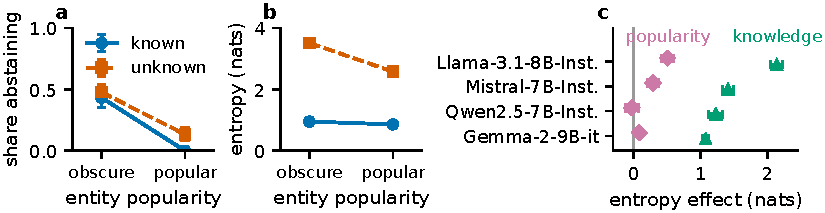
\includegraphics[width=\linewidth]{fig_dissociation.pdf}
\caption{\textbf{In Llama, saying \idk{} tracks popularity; answer entropy, a control, follows knowledge.} (a) Share of Llama's free replies both judges label \idk; (b) its first-token entropy when the reply must begin ``The answer is'' (values and $n$ in \cref{tab:cells}); (c) popularity and knowledge effects on that entropy in four instruct models. 95\% bootstrap intervals.}
\Description{Three panels. Abstention falls from obscure to popular entities for both known and unknown facts. Entropy separates known from unknown facts at both popularity levels. Across four instruct models, the knowledge effect on entropy exceeds the popularity effect.}
\label{fig:dissociation}
\end{figure}

With the two factors crossed, the first result is direct. On obscure entities whose facts it knows, Llama says \idk{} in \tcObsKnownAbs{} of replies; on popular entities whose facts it knows, it never does (\cref{tab:cells}). The answer distribution does not explain this: forced-answer entropy is similar in the two cells (\tcObsKnownEnt{} vs.\ \tcPopKnownEnt{} nats). The popularity effect on abstention is \hmLlamaPopEff{} \hmLlamaPopEffCI{} and the knowledge effect \hmLlamaKnowEff{} \hmLlamaKnowEffCI: a popularity preference of \hmLlamaDiff{} \hmLlamaDiffCI.

\begin{table}[t]
\caption{Llama-3.1-8B-Instruct by cell: share of free replies both judges label \idk, and forced-answer first-token entropy, with 95\% intervals; counts are for abstention, and entropy uses the full pool (\cref{app:robust}).}
\label{tab:cells}
\footnotesize\setlength{\tabcolsep}{4pt}\begin{tabular}{lcccc}
\toprule
& \multicolumn{2}{c}{Obscure} & \multicolumn{2}{c}{Popular} \\
\cmidrule(lr){2-3}\cmidrule(lr){4-5}
& known & unknown & known & unknown \\
\midrule
Says \idk{} & \tcObsKnownAbs{} \tcObsKnownAbsCI & \tcObsUnkAbs{} \tcObsUnkAbsCI & \tcPopKnownAbs{} \tcPopKnownAbsCI & \tcPopUnkAbs{} \tcPopUnkAbsCI \\
\quad questions & \tcObsKnownAbsN & \tcObsUnkAbsN & \tcPopKnownAbsN & \tcPopUnkAbsN \\
Entropy (nats) & \tcObsKnownEnt{} \tcObsKnownEntCI & \tcObsUnkEnt{} \tcObsUnkEntCI & \tcPopKnownEnt{} \tcPopKnownEntCI & \tcPopUnkEnt{} \tcPopUnkEntCI \\
\bottomrule
\end{tabular}
\end{table}

The other cells fit this. Llama abstains about as often on obscure facts it knows as on obscure facts it does not (\tcObsKnownAbs{} vs.\ \tcObsUnkAbs), and rarely on popular facts it does not know (\tcPopUnkAbs). This pattern is what the misfire idea predicts. But a contrast this sharp depends on how abstention and knowledge were measured, so we test both next.

\section{The Gap Replicates, but the Comparison Rests on a Few Relations}
\label{sec:holds}

We test the gap in the order a skeptical reader would: is it repeatable, are the obscure known facts really known, does it depend on the measure, and what does it rest on? \Cref{tab:robust} collects the estimates, and \cref{app:robust} gives each check in full.

\paragraph{The Gap Replicates.} With fresh replies, the preference is \frDiff{} \frDiffCI. In new questions from the 10th--30th and 70th--90th page-view percentiles, it is smaller but positive (\nqDiff{} \nqDiffCI), as the narrower contrast predicts.

\paragraph{Name Cues Do Not Explain It.} Replication does not show that Llama knows the obscure facts: it could guess them from the name. We re-asked each known question with three pseudo-names (two letters swapped, one vowel changed). Llama still answered \ncObsRec{} of \ncObsProbed{} obscure known facts correctly (\ncCountryRec{} of \ncCountryN{} country questions); these abstain less (\ncRecAbs) than the rest (\ncOtherAbs), and without them the preference is \ncDiff{} \ncDiffCI.

\paragraph{Other Labels Shrink It.} The labels themselves can also be wrong. Relabeling knowledge with a paraphrased question agrees with the original labels at $\kappa=\lcKappa$ (on the \lcBothN{} questions labeled under both); \eoObsKnownN{} of \gsObsKnownTotal{} obscure known facts stay known and abstain at \eoObsKnown, and the preference is \eoDiff{} \eoDiffCI. A larger model (Llama-3.3-70B) regraded popular unknown facts by meaning and moved \sePUKnown{} of 100 to known and \sePUInter{} to the dropped band; the preference becomes \seDiff{} \seDiffCI. Dropping every popular unknown question with the answer in any free reply (\lcPUAlias{} of them; post hoc) gives \lcAliasDrop{} \lcAliasDropCI. All label corrections at once (post hoc) leave \rcJoint{} \rcJointCI, while the gap among unknown facts stays \rcUnkJoint{} \rcUnkJointCI.

\paragraph{The Size Depends on the Measure.} The sign holds under six other measures of abstention, from \hjLlamaDiff{} to \faLlamaRegexDiff; we adopted the primary measure after the first pre-specified one returned the smallest of these. With a third judge the preference is \tjLlamaDiff; counting only replies that decline without naming any candidate, \sdDiff{} \sdDiffCI. These are refusals, not hidden answers: at most \lcDKAliasMax{} of \idk{} replies in any cell contain the gold answer (post hoc). Why the corrected judge and the regex disagree on the same replies is not established. A readout inside a single prompt is mixed. The pre-specified readout at the forced-answer position, the first token's lean toward hedge tokens (refusal openers such as `` I'', `` not'', `` unknown''), shows no preference (\loLlamaDiff{} \loLlamaDiffCI). A reading at the free prompt, specified after seeing this, shows one: popularity raises the log-odds of a first token ``I'' more than knowledge does (difference \eoFreeIDiff{} \eoFreeIDiffCI), while knowledge raises its entropy more (\eoFreeEntDiff{} \eoFreeEntDiffCI{} nats).

\paragraph{The Known-Fact Comparison Rests on a Few Relations.} Llama knows few obscure facts: \rcTopThree{} of the \gsObsKnownTotal{} come from three relations (capital, country, sport), as do \nqTopThree{} of \nqObsKnownN{} in the new questions. With relations as the resampling unit, the preference's interval is \rcClusCI{} (post hoc; leave-one-relation-out \rcLoro), while the gap among unknown facts stays clear (\rcUnkClusCI).

\begin{table}[t]
\caption{Llama's popularity preference under other measures of abstention and other knowledge labels, and the coefficient of the obscure arm under regression controls. Positive values mean abstention follows popularity more than knowledge. ``Corrected'': regex rates on 24-token replies corrected for the recall and precision of one LLM judge (Qwen2.5-32B-Instruct), measured on a subset labeled by that judge, not by people. Plan: pre-specified (pre) or post hoc. $n$: questions.}
\label{tab:robust}
\footnotesize\setlength{\tabcolsep}{3pt}\begin{tabular}{p{5.6cm}p{1.9cm}rll}
\toprule
Variant & Replies & $n$ & Plan & Estimate \\
\midrule
\multicolumn{5}{l}{\emph{Measures of abstention: popularity preference}} \\
Two judges, both DONT\_KNOW (primary) & 3, 96 tokens & \hmLlamaItems & pre & \hmLlamaDiff{} \hmLlamaDiffCI \\
Two judges, DONT\_KNOW or CLARIFY & same & \hmLlamaItems & pre & \hmLlamaSecDiff{} \hmLlamaSecDiffCI \\
Three judges, majority & same & \hmLlamaItems & pre & \tjLlamaDiff{} \tjLlamaDiffCI \\
70B judge, declines naming no candidate & same & \hmLlamaItems & pre & \sdDiff{} \sdDiffCI \\
Regex detector & same & \hmLlamaItems & post hoc & \hmLlamaRegexDiff{} \hmLlamaRegexDiffCI \\
Regex detector & 20, 24 tokens & \faLlamaN & pre & \faLlamaRegexDiff{} \faLlamaRegexDiffCI \\
One LLM judge, corrected & same 24-token & \faLlamaN & pre & \hjLlamaDiff{} \hjLlamaDiffCI \\
\midrule
\multicolumn{5}{l}{\emph{Replications and name-cue control (two judges): popularity preference}} \\
Fresh replies, same questions & 3, 96 tokens & \hmLlamaItems & pre & \frDiff{} \frDiffCI \\
New questions, 10th--30th vs.\ 70th--90th pct. & same & \nqN & pre & \nqDiff{} \nqDiffCI \\
Name-recoverable known facts removed & same & & pre & \ncDiff{} \ncDiffCI \\
\midrule
\multicolumn{5}{l}{\emph{Other knowledge labels (two judges): popularity preference}} \\
Relabeled with a paraphrased prompt & 3, 96 tokens & \lcBothN & pre & \eoDiff{} \eoDiffCI \\
\quad where both labelings agree & same & & post hoc & \lcCons{} \lcConsCI \\
Unknown facts regraded by meaning & same & & pre & \seDiff{} \seDiffCI \\
Popular unknown with the answer in a reply dropped & same & & post hoc & \lcAliasDrop{} \lcAliasDropCI \\
Guessable answers removed & same & & post hoc & \gsDiff{} \gsDiffCI \\
All label corrections jointly\textsuperscript{b} & same & & post hoc & \rcJoint{} \rcJointCI \\
\midrule
\multicolumn{5}{l}{\emph{Regression controls (two judges): coefficient of the obscure arm}} \\
Relation fixed effects and knowledge only & 3, 96 tokens & \hmLlamaItems & pre & \amObsBase \\
\quad plus entity recognition & same & \ekN & pre & \ekObs{} \ekObsCI \\
\quad plus namesake count & same & & post hoc & \amObs{} \amObsCI \\
\bottomrule
\end{tabular}

\smallskip\footnotesize \textsuperscript{b}Meaning-based regrade of unknown facts, popular unknown questions with the gold answer in any free reply dropped, and guessable facts removed. Relation-clustered 95\% intervals (resampling the 16 relations; post hoc): primary \rcClusCI, name-cue control \ncClusCI, new questions \nqClusCI; popularity gap among unknown facts \rcUnk{} \rcUnkClusCI.
\end{table}

So two results stand at different strengths. Llama abstains more on obscure entities, clearly so among facts it does not know. The stronger claim, that popularity beats knowledge, holds in every variant by point estimate, but its interval reaches zero once labels are corrected jointly or relations are resampled. Both are results about one model, which raises the next question.

\section{Gemma Shares the Preference When Permitted}
\label{sec:families}

\paragraph{Plain Prompt: Too Few Abstentions to Measure.} Entropy follows knowledge in all four families (\cref{fig:dissociation}c), but Qwen, Gemma and Mistral rarely say \idk; Gemma abstains in at most \tjGemmaObsUnk{} of replies per cell, so its preference cannot be estimated. A pre-specified four-family test found partial support for Qwen and Mistral (only the entropy condition holds), and full support for Gemma on a readout that shows no preference in Llama (\cref{app:families}).

\paragraph{Permissive Prompt: Same Preference in Gemma.} To obtain enough abstentions, we ended each question with ``If you do not know the answer, say that you do not know.'' Llama and Gemma then abstain often and three judges agree (Fleiss $\kappa=\pmLlamaKappa$ and \pmGemmaKappa). The popularity preference is \pmLlamaDiff{} \pmLlamaDiffCI{} for Llama and \pmGemmaDiff{} \pmGemmaDiffCI{} for Gemma, which says \idk{} to \pmGemmaObsKnown{} of obscure known and \pmGemmaPopKnown{} of popular known questions. For Qwen, Mistral and OLMo-2-7B, the judges disagree (Fleiss $\kappa$ \pmQwenKappa--\pmMistralKappa), so their preferences are unmeasured (point estimates \pmQwenDiff, \pmMistralDiff, \pmOlmoDiff; \cref{app:families}).

The preference therefore appears in the two families where we can measure it, and we cannot say more about the others. Two models sharing a behavior does not tell us why it happens. If the cause is familiarity, the model should represent obscure names as unfamiliar, and a popularity direction should do something an abstention direction does not. We test both.

\section{No Familiarity Mechanism Isolated}
\label{sec:mech}

\paragraph{Obscure Names Do Not Look Unfamiliar to Llama.} Entity recognition, an LLM-graded test of whether Llama can describe the entity, averages \ekObsKnown{} for obscure known facts and \ekPopKnown{} for popular known ones, and shrinks the popularity coefficient by \ekShrink. Wikidata name collisions (post hoc) leave it at \amObs{} \amObsCI. Mean name surprisal under base Llama is uncorrelated with log page views (Spearman \esRho), so it does not stand in for popularity. Name form explains part of the gap: between \scPopKnownPairs{} matched pairs of known facts, the regex abstention gap of \scPopKnownGap{} shrinks to \scPopKnownGapSurface{} \scPopKnownGapSurfaceCI{} once the names' word frequency, token count and token rarity are held equal (post hoc).

\begin{figure}[t]
\centering
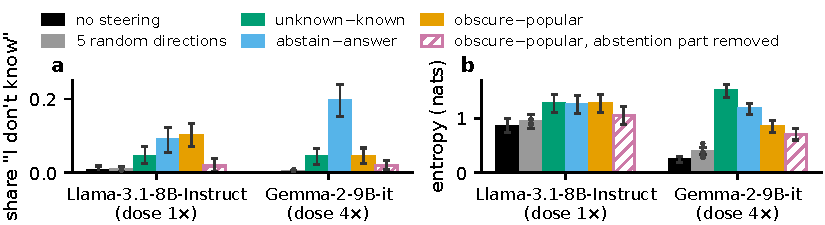
\includegraphics[width=\linewidth]{fig_steering.pdf}
\caption{\textbf{In Llama, steering along the obscure-minus-popular direction adds little abstention beyond its overlap with an abstention direction.} Each bar adds one direction to the residual stream at a dose chosen on separate questions (1$\times$ its natural norm for Llama, 4$\times$ for Gemma) and is scored on 150 held-out popular questions the model knows. (a) Share of free replies both judges label \idk. (b) First-token entropy under the forced-answer prompt. Grey: mean of 5 random directions (dots: each direction). Hatched: obscure-minus-popular with its abstain-minus-answer component removed. Gemma's judges agree below the pre-specified bar, so its bars in (a) are indicative only. Error bars: 95\% bootstrap over questions.}
\Description{Two bar panels for Llama and Gemma. In Llama, the obscure-minus-popular direction raises the share saying I don't know, and removing its abstention component returns it near the random level. Entropy rises under all fitted directions.}
\label{fig:steering}
\end{figure}

\paragraph{Steering Finds a Generic Abstention Signal.} Like work steering refusal along recognition directions \cite{ferrando2025iknow,brzezinka2026familiarity}, we fitted obscure-minus-popular, unknown-minus-known and abstain-minus-answer directions on half of the questions \cite{arditi2024refusal,rimsky2024caa}, chose the dose on a second set of popular known questions and scored a third (\cref{fig:steering}, \cref{app:steer}). In Llama, obscure-minus-popular adds \svLlamaDOne{} \svLlamaDOneCI{} abstention over random directions (short of the pre-specified $+0.10$ bar). It is nearly parallel to abstention directions fitted without any popularity contrast: cosine \wlLlamaCos{} for one fitted on obscure questions only and \gaCos{} for one fitted on popular questions only. Removing either leaves \wlLlamaDTwo{} \wlLlamaDTwoCI{} and \gaPerp{} \gaPerpCI. It beats unknown-minus-known on abstention (\svLlamaDThree), as the cells' rates predict; in Gemma, unknown-minus-known raises entropy \svGemmaDFour{} \svGemmaDFourCI{} nats more (\cref{fig:steering}b; cf.\ \cite{che2026steering}). The popularity direction therefore moves abstention without showing a popularity-specific route.

\paragraph{Lenses Show Both Factors in Base Models.} With prefitted Jacobian lenses \cite{gurnee2026workspace}, read at the forced-answer position in a pre-specified mid-depth window, popularity raises the hedge-token term in Llama-3.1-8B, Gemma-2-9B, Gemma-2-2B and OLMo-3-7B \cite{olmo3}, and knowledge raises it comparably or more in three of four (\cref{tab:lens}). Instruct partners lean further toward knowledge, so this readout does not show where Llama-Instruct's preference arises. The pre-specified prediction that popularity's effect starts at a shallower depth than knowledge's was not supported (\jlSupports{} supporting, \jlContradicts{} contradicting and \jlUndecided{} undecided of the eight base and instruct models).

\section{Limitations}

Abstention is judged by LLMs not validated against human labels; their errors could differ by cell and could bias the preference in either direction. ``Known'' is specific to the forced-answer prompt and concentrated in three relations. The design contrasts extreme deciles, and the adjacent bands give a smaller preference. Popularity is a stand-in that also carries name form. The models have 2--9B parameters, and only two families could be measured. Hedging driven by ambiguity that the judges do not label as clarification is not excluded.

\section{Conclusion}

We began by asking what a model's \idk{} responds to. In Llama, on these questions, it responds to how popular the entity is more than to whether the model can give the answer: \tcObsKnownAbs{} on obscure facts it knows, \tcPopUnkAbs{} on popular facts it does not. The comparison between the two factors is suggestive rather than settled, since it shrinks to \rcJoint{} \rcJointCI{} under joint label corrections and rests on three relations. The popularity gap among unknown facts is firmer. Gemma shows the same preference when the prompt permits abstaining.

\emph{Interpretation:} the result has the shape the misfire idea predicts, but we did not establish its mechanism. Our measures do not show obscure names to be unfamiliar, and steering isolates only a generic abstention signal. Surface features of names and instruction tuning remain open alternatives, and more investigation is needed.

\emph{Recommendation:} an evaluation that reads abstention as a measure of what a model does not know should cross it with entity popularity and report per-cell rates. Here, a single abstention rate would hide that the same statement is common on obscure facts the model knows and rare on popular facts it does not.


\appendix

\section{Robustness Checks in Full}
\label{app:robust}

\emph{Design counts.} Llama's pool has \lkObsPoolKnown{} known, \lkObsPoolMaybe{} intermediate and \lkObsPoolUnk{} unknown obscure facts, and \lkPopPoolKnown{}, \lkPopPoolMaybe{} and \lkPopPoolUnk{} popular ones; the two-judge sample is a stratified random sample of 100 questions per cell (seed 0), or all of a smaller cell. Intervals for differences of cell means use 10,000 within-cell bootstraps (seed 0); linear probability models use 2,000 bootstraps over questions.

\emph{Measurements.} The single corrected judge gives the smallest difference. Its 24-token replies are often cut off before the model commits; why it and the regex disagree on the same replies is not established. The two-judge measurement with 96 tokens was designed for that reason after the \hjLlamaDiff{} was seen and made primary before it ran.

\emph{Independent labels} (pre-specified). Knowledge was relabeled with one paraphrased question per relation, the assistant prefix ``Answer:'' and fresh samples, under the same rule. Of the \lcBothN{} questions labeled under both prompts, \lcKK{} are known under both, \lcUU{} unknown under both, \lcKU{} known only originally and \lcUK{} only under the paraphrase (agreement \lcAgree, $\kappa=\lcKappa$). Where both labelings agree, cells have \lcConsN{} questions (obscure unknown, obscure known, popular unknown, popular known). Under the new labels, the popularity effect on abstention is \eoPop{} \eoPopCI{} and the knowledge effect \eoKnow{} \eoKnowCI, and original-prompt entropy follows them (knowledge minus popularity \eoEntKmP{} \eoEntKmPCI).

\emph{Entity recognition} (pre-specified). Llama completed ``\{subject\} is'' after the question ``What is \{subject\}?'' (greedy and five samples), and Llama-3.3-70B graded each completion against the subject's English Wikidata description; recognition is the share of completions graded correct. It averages \ekObsKnown{} for obscure known facts and \ekPopKnown{} for popular known facts.

\emph{Guessable answers} (post hoc). An answer counts as guessable if a gold alias of at least three characters appears in the subject's name, or if it is its relation's most common answer and covers at least 20\% of the relation's pool. By this rule \rcGuessN{} of the \gsObsKnownTotal{} obscure known facts are guessable; they abstain at \rcGuessAbs, and the other \rcNonGuessN{} at \rcNonGuessAbs.

\emph{Free replies} (post hoc). Counting a gold alias only when it is not part of the subject's name, \ecAll{} of the free replies in the obscure known cell contain the answer, as do \ecNonAbs{} of the replies that do not abstain and \ecAbs{} of those that do (popular known: \ecPopKnown). For \ecBoth{} of \ecBothOf{} obscure known questions, one free reply gives the answer and another says \idk.

\section{Other Families}
\label{app:families}

The pre-specified four-family test asked whether hedging follows popularity more than knowledge and entropy follows knowledge more than popularity, each on a fixed hedging readout: the regex on 24-token free replies for Llama (the reference, where both hold), Qwen and Mistral (only the entropy condition holds), and, because Gemma's replies rarely hedge, the forced-answer hedge log-odds for Gemma (both hold, although this readout shows no preference in Llama).

\emph{Permissive prompt} (pre-specified). The user message was the question followed by ``If you do not know the answer, say that you do not know.'', on each model's existing two-judge question set, with three replies scored by the three judges and a majority rule. Cell rates (obscure unknown, obscure known, popular unknown, popular known): Llama \pmLlamaObsUnk, \pmLlamaObsKnown, \pmLlamaPopUnk, \pmLlamaPopKnown; Gemma \pmGemmaObsUnk, \pmGemmaObsKnown, \pmGemmaPopUnk, \pmGemmaPopKnown. Qwen2.5-7B, Mistral-7B and OLMo-2-7B-Instruct (pre-specified; OLMo on its own pool, obscure known $n=48$) are unmeasured under the same rule (Fleiss $\kappa$ \pmQwenKappa, \pmMistralKappa, \pmOlmoKappa); their point estimates are \pmQwenDiff{} \pmQwenDiffCI, \pmMistralDiff{} \pmMistralDiffCI{} and \pmOlmoDiff{} \pmOlmoDiffCI. The criterion let Gemma's verdict replace ``cannot be estimated'' only if its obscure unknown rate reached 0.25.

\section{Steering}
\label{app:steer}

Pre-specified. Directions were fitted on a random half of each model's questions at layer round$(0.55\times(L-1))$, the last position of the free prompt: obscure minus popular and unknown minus known (differences of cell means, each averaged over the other factor), and abstain minus answer (questions whose stored free-generation regex abstention rate is at least 0.5 minus those with rate 0). The obscure-minus-popular direction with its abstention component projected out was rescaled to the original norm. Each direction was added at a dose $k\in\{0.5,1,2,4,8\}$ times the obscure-minus-popular direction's natural norm, at the last prompt position and every generated position. $k$ was chosen on 150 popular known questions as the smallest value at which that direction beat five random directions by 0.10 in regex abstention, a rule separate from the confirmatory bar (\svLlamaDose$\times$ for Llama, \svGemmaDose$\times$ for Gemma, whose obscure-minus-popular regex rate was \svGemmaSelOne{} at 1$\times$ and \svGemmaSelTwo{} at 2$\times$). All conditions were scored on 150 further popular known questions, \lkSteerOverlap{} of which are also in the two-judge sample.

Primary scorer (both judges), obscure-minus-popular minus random: Llama \svLlamaDOne{} \svLlamaDOneCI, Gemma \svGemmaDOne{} \svGemmaDOneCI; with abstention removed: \svLlamaDTwo{} \svLlamaDTwoCI{} and \svGemmaDTwo{} \svGemmaDTwoCI; obscure-minus-popular minus unknown-minus-known: \svLlamaDThree{} \svLlamaDThreeCI{} and \svGemmaDThree{} \svGemmaDThreeCI. Secondary scorer (a majority of three judges, added by amendment before judging): obscure-minus-popular minus random \svLlamaMajDOne{} \svLlamaMajDOneCI{} and \svGemmaMajDOne{} \svGemmaMajDOneCI; with abstention removed \svLlamaMajDTwo{} \svLlamaMajDTwoCI{} and \svGemmaMajDTwo{} \svGemmaMajDTwoCI. For Gemma the secondary scorer is the defensible one, since its two judges agree below the bar. The cosine between the obscure-minus-popular and abstention directions is \svLlamaCos{} in Llama and \svGemmaCos{} in Gemma. No condition produced degenerate text.

\emph{Popular-arm abstention direction} (pre-specified). To test whether the overlap is with abstention in general, the abstain-minus-answer direction was refitted on popular questions only (\gaHi{} abstaining against \gaLo{} answering), with 20 random directions instead of 5, and scored by a majority of three judges (Llama, dose 1). Its cosine with obscure-minus-popular is \gaCos. Over random directions it adds \gaAbst{} \gaAbstCI, obscure-minus-popular adds \gaFam{} \gaFamCI, and obscure-minus-popular with this direction removed adds \gaPerp{} \gaPerpCI: the obscure-minus-popular direction adds no abstention beyond its overlap with an abstention direction fitted without any obscure entities.

\section{Lens and Name Surprisal}
\label{app:lens}

Pre-specified. Hedge term: log-sum-exp of the lens log-probabilities of the hedge tokens `` not'', `` I'', `` unknown'', `` unclear'' and `` no''; the full readout subtracts the same quantity for the answer-opening tokens `` a'', `` the'', `` that'', `` in'', `` Yes'' and `` yes''. Window: relative depth $\ell/(L-1)\in[1/3,2/3]$. Intervals: 2,000 within-cell bootstraps. Each model was labeled known or unknown on its own prompt with the same sampling rule.

\begin{table}[h]
\caption{Mid-depth window effects in base models, with 95\% intervals. Lenses are fitted per model, so compare effects within a model, not across models.}
\label{tab:lens}
\scriptsize\setlength{\tabcolsep}{3pt}\begin{tabular}{lcccc}
\toprule
& \multicolumn{2}{c}{Full readout} & \multicolumn{2}{c}{Hedge term alone} \\
\cmidrule(lr){2-3}\cmidrule(lr){4-5}
Model & Popularity & Knowledge & Popularity & Knowledge \\
\midrule
\lwRows
\bottomrule
\end{tabular}
\end{table}

\emph{Instruct partners} (pre-specified). The same readout, window and labeling rule were applied to Llama-3.1-8B-Instruct, Gemma-2-9B-it and Gemma-2-2B-it with their own prefitted lenses and chat-template forced-answer prompts. The criterion allowed the claim that instruction tuning increases the popularity preference only if, for a pair, the instruct difference exceeded the base difference with non-overlapping intervals; this held for no pair.

\emph{Name surprisal} (pre-specified). We computed the mean per-token surprisal of each subject name under the base Llama-3.1-8B in the context ``Here is a name:''. It is uncorrelated with log page views (Spearman \esRho). Surprisal therefore does not stand in for popularity. Short names made of common words (``New York'' as a book title) are a likely reason.


\bibliographystyle{ACM-Reference-Format}
\bibliography{../references}

\end{document}
